\chapter{Preliminary Concepts: Taming Velocity and Variety}\label{ch:background}

\textcolor{red}{FINAL - TO BE READ ONE LAST TIME}

The transient nature of streaming data often requires to treat it differently from persistent data, which can be stored and queried on demand. Data streams should often be consumed on the fly by continuous queries. Such a paradigmatic change has been largely investigated in the last decade by the database community~\cite{garofalakis2016data}, and, more recently, by the Semantic Web community~\cite{della2009s}. Several independent groups have proposed extension of RDF and SPARQL~\cite{w3c_sparql} for continuous querying~\cite{Barbieri2010b,DBLP:conf/semweb/PhuocDPH11,DBLP:conf/semweb/CalbimonteCG10} and reasoning~\cite{DBLP:journals/ijsc/BarbieriBCVG10,Anicic2011}. 

\sloppy The development of these solutions needs to deal with the nature of data streams and with the user needs. 
The input information always changes over time \textit{(Velocity)}, the sources are different and offer data that vary in syntax, structure and semantics \textit{(Variety)}. The data continuously flows into the system and, even what looks like \textit{static data}, e.g. a city street grid, is not immutable over time. It slowly evolves.

In the next sections, we present an overview on (i) the theoretical and practical concepts developed for managing data characterized by velocity and variety, (ii) the solutions to easy the creation of system based on RDF Stream Processors, and (iii) the benchmarking principles and techniques.
In the Section~\ref{sec:velocity}, we present the theoretical models, the languages and the architectures for taming velocity, and we conclude with an overview of the extended solutions we exploited during the research work. Section~\ref{sec:variety} presents an overview on the concepts and the architectures for managing the variety.
In Section~\ref{sec:vel-var}, we present an overview on the attempts for taming both velocity and variety in a single architecture.
In Section~\ref{sec:rsp-mid}, we present the fundamental principles of an RSP middleware and the implementations we exploited as term of comparison during this work.
Finally, Section~\ref{sec:benchmarking} presents the benchmarking principles and the benchmarking techniques and metrics we exploited during this research work.

\section{Velocity}\label{sec:velocity}
Section~\ref{sec:stream-proc} presents an overview of the models and languages to manage the data velocity. Sections \ref{sec:vel-arch} and \ref{sec:vel-sol} then present two different architecture for a velocity-first system, and the solutions that inspired our research work.

\subsection{Models and Languages}

\subsubsection{Stream Processing} \label{sec:stream-proc}
In order to introduce the concepts related to the analysis of streaming data, we need to introduce the concepts of Time and Time Instant.

\begin{Definition}
(Time) The time Ti is an infinite, discrete, ordered sequence of time instants $(t_1,t_2,..., t_n)$, where $t_i \in \mathbb{N}$. A time unit is the difference between two consecutive time instants $(t_{i+1} - t_i)$ and it is constant.
\end{Definition}

\begin{Definition}
(Time Instant) A time instant (or simply instant) is any value from T.
\end{Definition}

Now that we have formally defined the Time concept, we can introduce the Stream.

\begin{Definition}
(Stream) A stream S is a bag (multiset) of elements $\langle s,\tau \rangle$, where s is a tuple belonging to the schema of S and $\tau \in Ti$ is the timestamp of the element.
\end{Definition}

This definition of stream does not consider the time as a part of the data schema. 
At any time instant $\tau \in Ti$, zero or more elements could be in the stream and, consequently, share the timestamp.

We finally present a formal definition of Relation, an unordered bag of tuples at any time instant $\tau \in Ti$, or simply $R(\tau)$.

\begin{Definition}
(Relation) A relation R is a mapping from T to a finite but unbounded bag of tuples belonging to the schema of R.
\end{Definition}
 
\subsubsection{CQL}\label{sec:CQL}
The Continuous Query Language(CQL)~\cite{arasu2006cql} represents both an expressive SQL-based declarative language for managing continuous queries against streams and updatable relations, and a processing model. 
It was originally proposed by the DB group of the Stanford university.

\begin{figure}[h]
  \begin{center}
    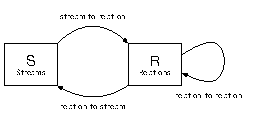
\includegraphics[width=.65\textwidth]{img/cql-model}\\
    \caption{The CQL processing model.}
    \label{fig:cql-model}
  \end{center}
\end{figure}

Figure~\ref{fig:cql-model} depicts the three operators defined by the CQL processing model. 
\begin{itemize}
\item[(i)] The stream-to-relation. It takes a stream S as input and produces a relation R as output, maintaining the schema. At any instant~$\tau$, $R(\tau)$ should be computable from S.
\item[(ii)] The relation-to-relation operator. It takes one or more relations $R_1,... , R_n$ as input and produces a relation R as output. At any instant $\tau$, $R(\tau)$ should be computable from $R_1(\tau),... , R_n(\tau)$.
\item[(iii)] The relation-to-stream operator. It takes a relation R as input and produces a stream S as output maintaining the schema. At any instant $\tau$, S at $\tau$ should be computable from R up to $\tau$.
\end{itemize}

CQL, also, define an abstract semantics for the data management:
\begin{Definition}
(Continuous semantics) Consider a query Q that is a composition of the three basic CQL operators. 
The inputs to the operators operators of Q are streams $S_1, ..., S_n (n \geq 1)$ and relations $R_1,..., R_m (m \geq 0)$. 
The result of continuous query Q at a time $\tau$ when all inputs are "available" can be defined as:
\begin{enumerate}
\item If the top operator in Q is relation-to-stream and produces the stream S, the result of Q at time $\tau$ is S up to $\tau$, produced by recursively applying the operators comprising Q to streams $S_1, ..., S_n$ up to $\tau$ and relations $R_1,..., R_m$ up to $\tau$.
\item If the top operator in Q is stream-to-relation or relation-to-relation and produces the relation R, the result of Q at time $\tau$ is $R(\tau)$, produced by recursively applying the operators comprising Q to streams $S_1, ..., S_n$ up to $\tau$ and relations $R_1,..., R_m$ up to $\tau$.
\end{enumerate}
\end{Definition}

\paragraph{Stream-to-relation operators}
The stream-to-relation operators in CQL are based on the sliding window concept (see Section \ref{sec:rsp-ql}). CQL exploits the concepts of window to define three classes of sliding window: time-based, tuple-based and partitioned.

\begin{Definition}
(Window) A window $W(S)$ is a set of elements extracted from a stream S. 
\end{Definition}

Time-based sliding window operator's output is defined by sliding an interval of T time units over the stream $S$. 
\begin{Definition}
(Time-based sliding window) A time-based sliding window on a stream S takes a time-interval T as a parameter and is specified by following S in the query with [Range T].
The output relation R of S[Range T] is defined as:
\noindent\begin{align*}
R(\tau)=\{s \mid \langle s,\tau' \rangle \in S \wedge (\tau' \leq \tau) \wedge (\tau' \geq \max\{\tau - T,0\})\}
\end{align*}  
\end{Definition}

Tuple-based sliding window operator's output is defined by sliding a window of size N tuples over the stream $S$.
\begin{Definition}
(Tuple-based sliding window) A tuple-based sliding window takes a positive integer N as a parameter and is specified by following S in the query with [Rows N].
The relation R of S[Rows N], R($\tau$), consists of tuples obtained from the N elements with the largest timestamps in S no greater than $\tau$.
\end{Definition}

Partitioned sliding window logically partitions $S$ into different sub-streams based on equality of attributes $A_1, ..., A_k$, computes a tuple-based sliding window of size $N$ on each sub-stream, then the output relation is the union of these sub-windows.
\begin{Definition}
(Partitioned sliding window) A partitioned sliding window on a stream S takes a positive integer N and a subset $\{A_1, ..., A_k\}$ of S attributes as parameters. It is specified by following S in the query with [Partition By $A_1, ..., A_k$ Rows N].
Formally, a tuple s with values $a_1, ..., a_k$ for attributes $A_1, ..., A_k$ occurs in output instantaneous relation R($\tau)$ iff exists an element $\langle s,\tau' \rangle \in S$ such that $\tau' \leq \tau$ is among the N largest timestamps among elements whose tuples have values $a_1, ..., a_k$ for attributes $A_1, ..., A_k$
\end{Definition}

\paragraph{Relation-to-relation operators}
The relation-to-relation operators operators transform relations in other relations. 
They are often derived from typical relational queries, by applying the semantic mapping to time-varying relations.
Relational algebraic expressions are a well-known cases of this class of operators.

\paragraph{Relation-to-stream operators}
Starting from the concepts of stream and relation, CQL defines three classes of relation-to-stream operators: Istream, Dstream, and Rstream. 

\begin{Definition}
(Istream) The insert stream applied to relation R contains an element $\langle s,\tau \rangle$ iff the tuple s is in $R(\tau) - R(\tau - 1)$: 
\noindent\begin{align*}
Istream(R) = \bigcup_{\tau \geq 0} ((R(\tau) - R(\tau - 1)) \times \{\tau\}).
\end{align*} 
\end{Definition}

\begin{Definition}
(Dstream) The delete stream applied to relation R contains an element $\langle s,\tau \rangle$ iff the tuple s is in $R(\tau - 1) - R(\tau)$: 
\noindent\begin{align*}
Dstream(R) = \bigcup_{\tau \geq 0} ((R(\tau - 1) - R(\tau)) \times \{\tau\}).
\end{align*} 
\end{Definition}

\begin{Definition}
(Rstream) The relation stream applied to relation R contains an element $\langle s,\tau \rangle$ iff the tuple s is in $R$ at time $\tau$: 
\noindent\begin{align*}
Rstream(R) = \bigcup_{\tau \geq 0} (R(\tau) \times \{\tau\}).
\end{align*} 
\end{Definition}

The concepts introduced by CQL represent a fundamental theoretical base for the development of the stream processors, see Section~\ref{sec:vel-var-solutions}. We exploited these constructs during the development of our Streaming Computational Model, see Chapter~\ref{ch:computational}.  

\subsubsection{SECRET}\label{sec:secret}
In 2000s, different systems try to implement a streaming processing model (see Section~\ref{sec:vel-var-solutions}). Despite they are based on common concepts, they present significant differences in the way they manage data and queries.
In order to explain the differences in the behavior of window operators in the existing stream processing engines, Botan et el. present SECRET~\cite{DBLP:journals/pvldb/BotanDDHMT10}.
Differently from CQL, it assigns two time instants to each stream item: (i) the application and (ii) the system time. The former, already defined by CQL processing model, refers to the instant related to the event represented by the element in the stream. It is not unique (contemporaneity is allowed) and defines a partial order among the stream elements. The latter must be unique and introduces a total order in the stream. From a conceptual point of view, the application time represents the most relevant information, but the system time is also important to understand the correct behavior of the stream engine.

\begin{figure}[h]
  \begin{center}
    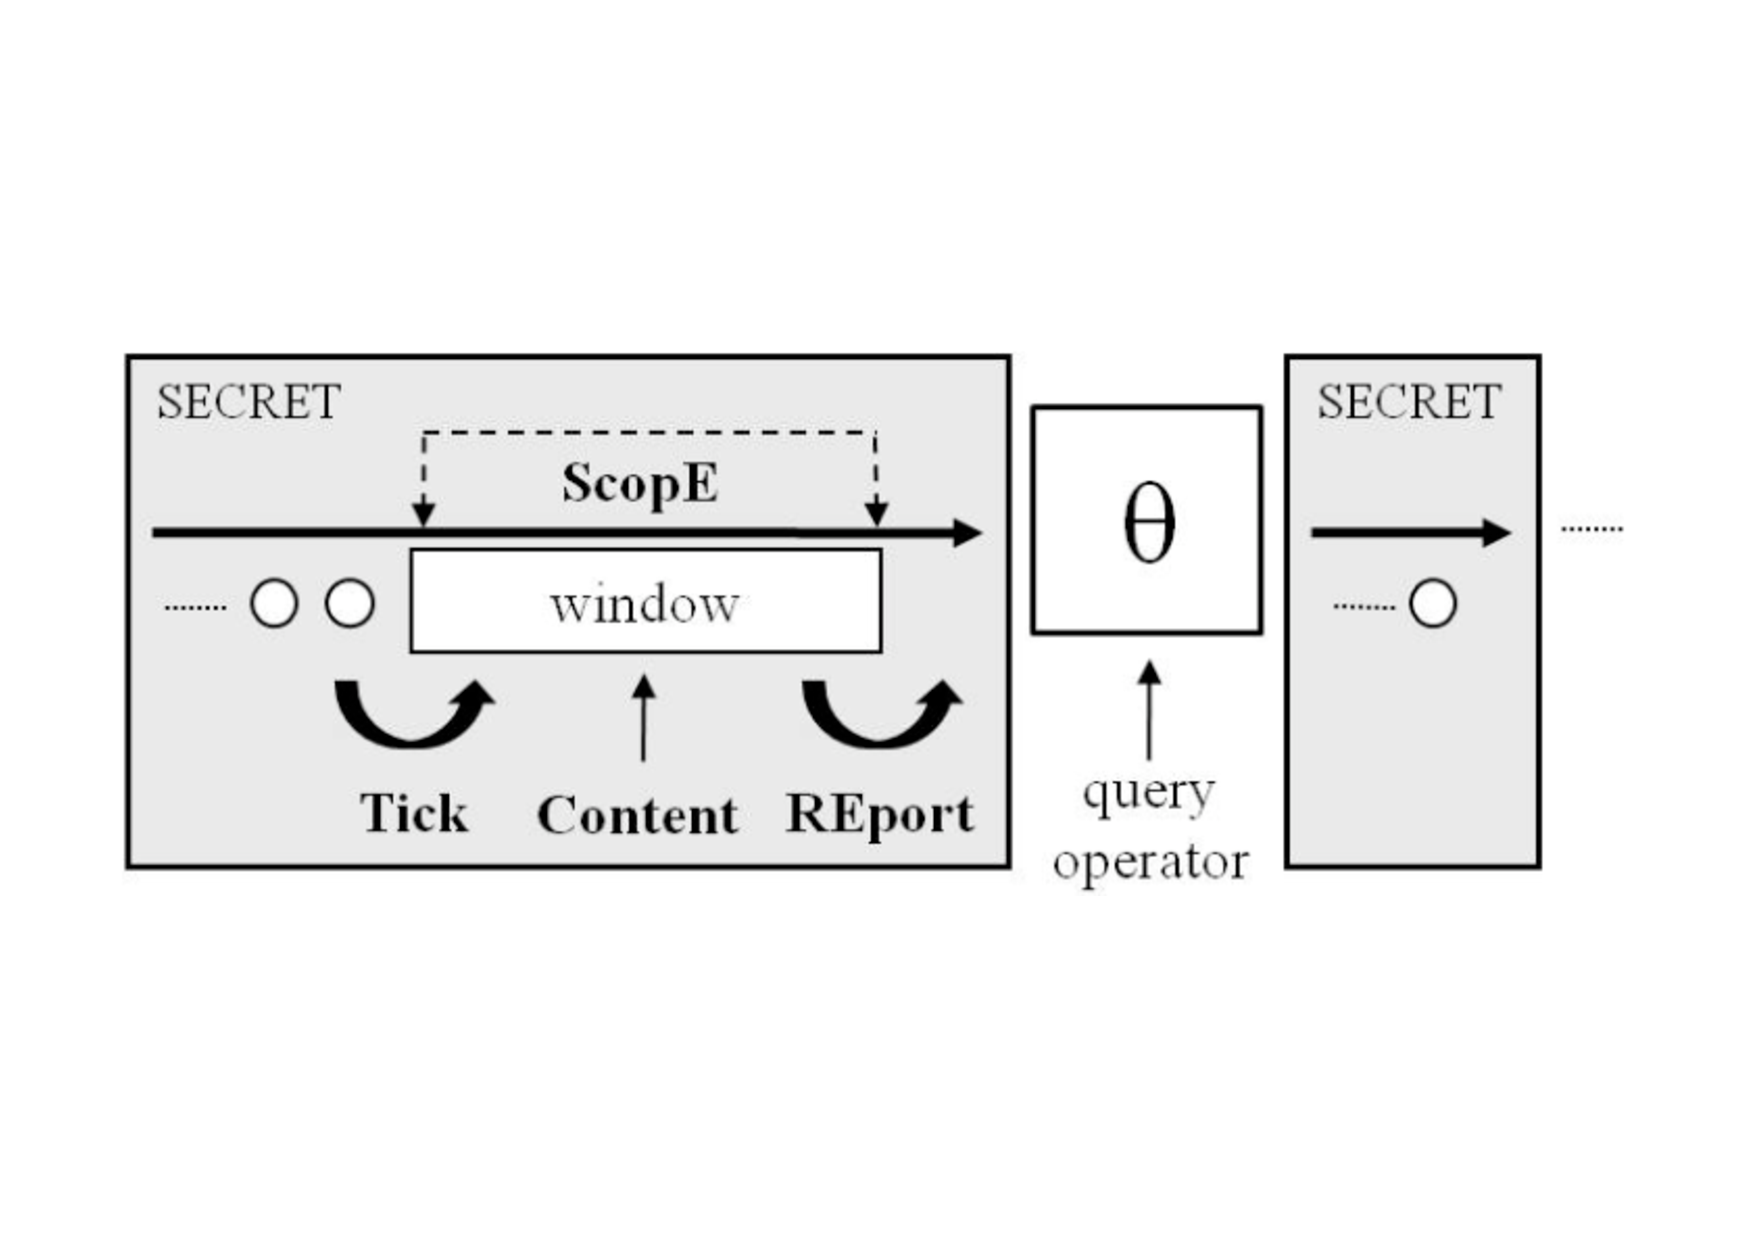
\includegraphics[width=0.8\textwidth]{img/secret}\\
    \caption{SECRET of a query plan (source \cite{DBLP:journals/pvldb/BotanDDHMT10}).}
    \label{fig:secret}
  \end{center}
\end{figure}

As depicted in Figure~\ref{fig:secret}, the SECRET framework introduces the notions of scope, content, report and tick to explain the window operator.

The \textit{Scope} function associates an evaluation time instant $t$ to the active window time interval. The computation of the scope relies on the $t_0$ parameter, the first active window start timestamp.

The \textit{Content} identifies the set of items of S in the active window. This function is influenced by both the application and the system time.

The \textit{Report} function defines the conditions under which the relation-to-relation operators can access the window content for additional query evaluation and result reporting. SECRET identifies four reporting strategies: (i) Content change -- the system reports if the content changes --, (ii)  Window close -- the system reports if the active window closes --, (iii) Non-empty content -- the system reports if the active window is not empty -- and, finally, (iv) Periodic -- the system reports only at regular intervals.

The \textit{Tick} is a function that defines under which conditions input can enter the window and, consequently, can be processed by the engine. SECRET defines tuple-driven and time-driven strategies. Systems that adopt the former strategy add the tuple to the window operator as soon as they arrive, contrariwise, systems that adopt the latter strategy, add tuple to the window at each application time instant.

The key concepts formalized by SECRETS result useful to guarantee a comparable behavior of all the different implementations of our Conceptual Model presented in Chapter~\ref{ch:computational}.

\subsection{Information Flow Processing and Architectures}\label{sec:vel-arch}
% This section introduces the information flow processing (IFP)~\cite{DBLP:journals/csur/CugolaM12}, an application domain in which, data from multiple distributed sources, needs to be processed in order to extract knowledge as soon as the relevant information is collected.
% In particular, we limit the overview to the IFP functional model (presented in the Section~\ref{sec:ifp-fm}), because it can be considered the foundation of the $\kappa$ architecture (see Section~\ref{sec:k-arch}) and $\lambda$ architecture (see Section~\ref{sec:l-arch}), that describe, from an higher point of view, the organization of a data processing architecture including stream processing components. 

Cugola et al. in~\cite{DBLP:journals/csur/CugolaM12} proposed the Information Flow Processing (IFP) as an application domain in which users need to collect information produced by multiple, distributed sources for processing it in a timely way in order to extract new knowledge as soon as the relevant information is collected.

From an high-level point of view, an IFP takes data flows from multiple sources as input, processes them and produces other information flows as output. This output is then directed toward a set of sinks.

\begin{figure}[h]
  \begin{center}
    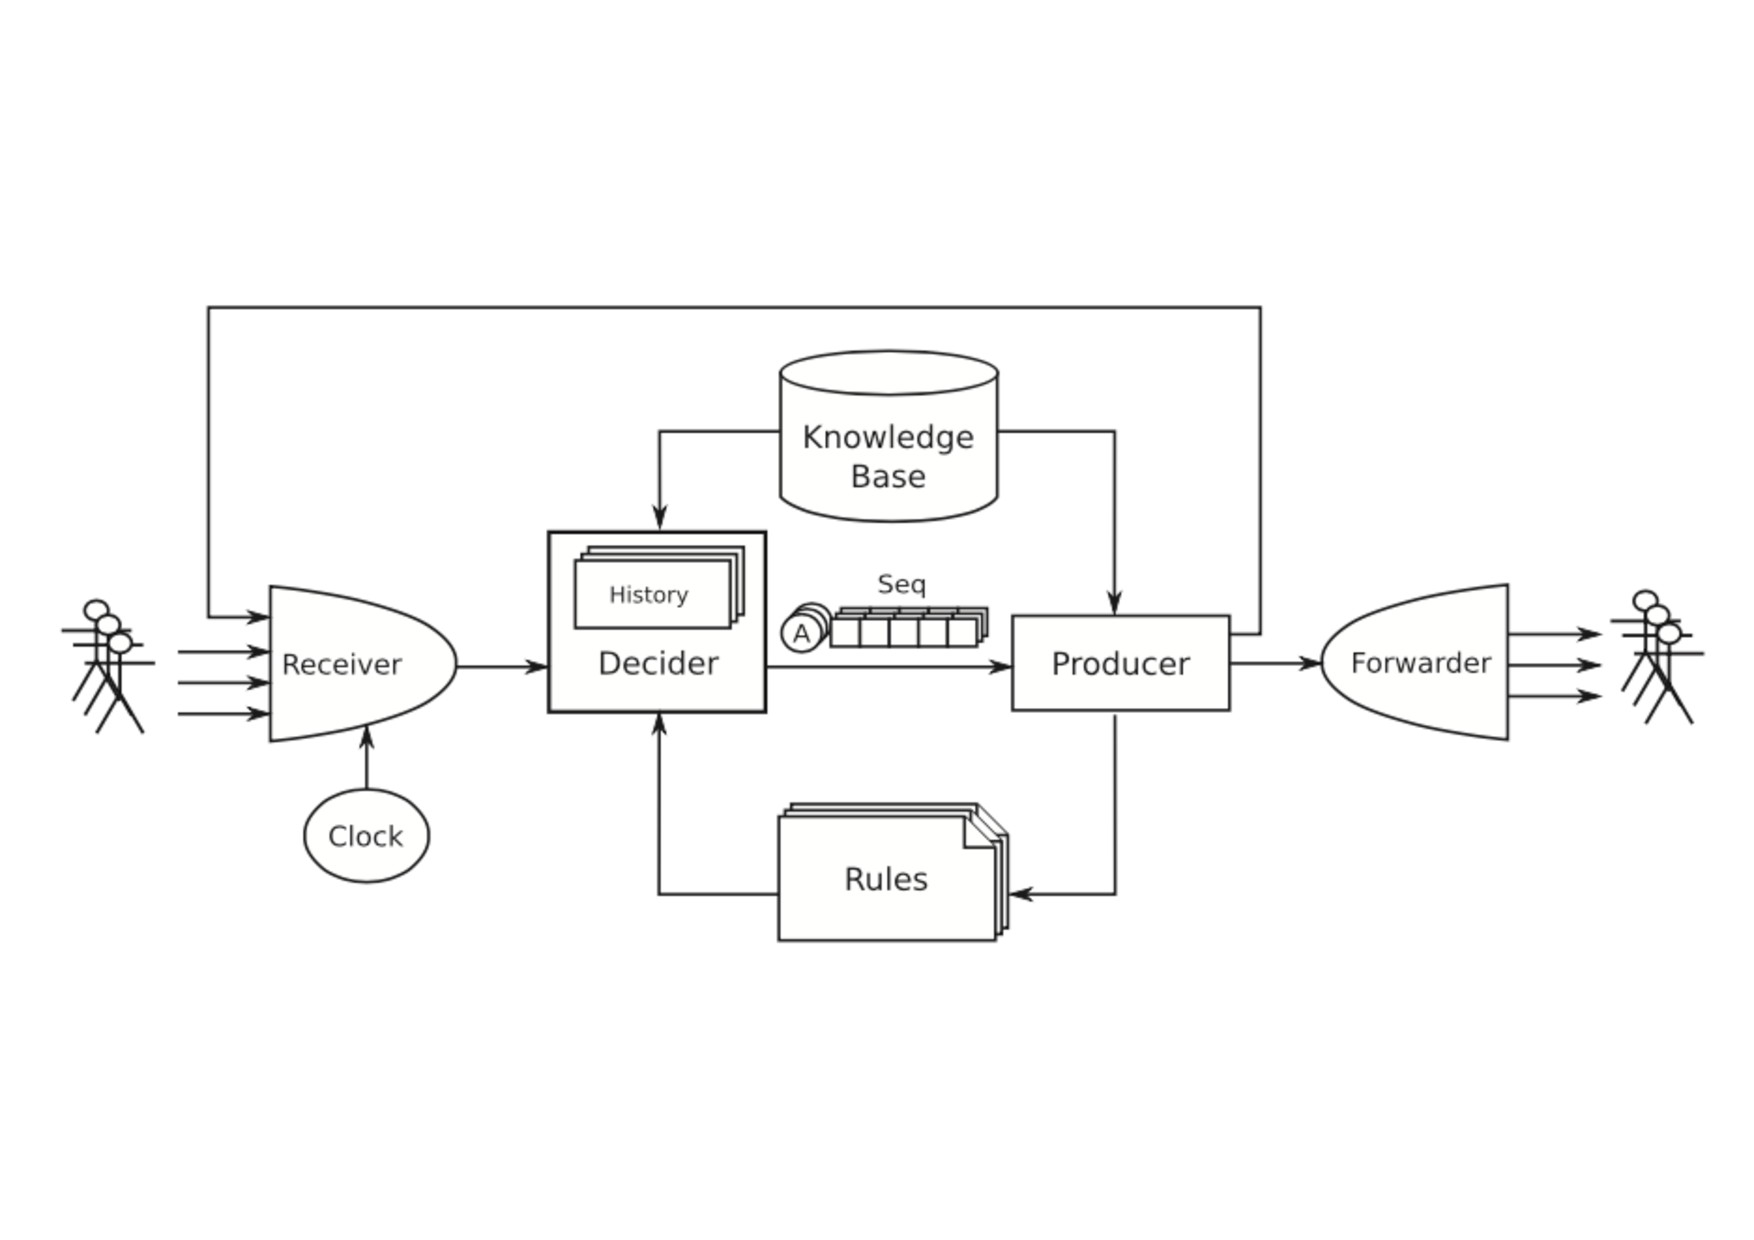
\includegraphics[width=\textwidth]{img/ifp}
    \caption{The functional architecture of an IFP system (source \cite{DBLP:journals/csur/CugolaM12}).}
    \label{fig:ifp}
  \end{center}
\end{figure}

Figure~\ref{fig:ifp} shows the components of a generic IFP system.
The \textit{receiver} implements the transport protocol to move data over the network and manages the connection between the sources and the IFP engine. Moreover, it is also connected to the \textit{clock} -- an architectural element that produces special data items that hold the current time.
Then, the data items, from external sources or from the clock, enter the processing pipeline that elaborates the data according to the rules stored into the rule store.
A rule is logically composed by a condition part (C) and an action part (A). C specifies the condition that has to be satisfied by the information to trigger the rule in the IFP, while A specifies what to do. The logical disjunction produces a physical disjunction, the processing are splitted in two different phases: (i) the detection -- realized by the \textit{decider} that checks the condition (C) on each incoming item --, and (ii) the production -- realized by the \textit{producer} that triggers the actions (A).
The \textit{knowledge base} represents a read only-memory\footnote{The knowledge base is read-only from the IFP engine perspective, but can be modified by external systems} that contains useful information for the decider and the producer.
Finally, the \textit{forwarder} is in charge to deliver the information to the output sinks.

In the early 2010s, Nathan Marz coined the term $\lambda$ architecture describing a generic, scalable and fault-tolerant data processing architecture that was very successful in distributed environment. 
The IFP functional model are at the basis of this architecture, formalizes by Marz et al. in ~\cite{marz2015big}.

\begin{figure}[t]
  \begin{center}
    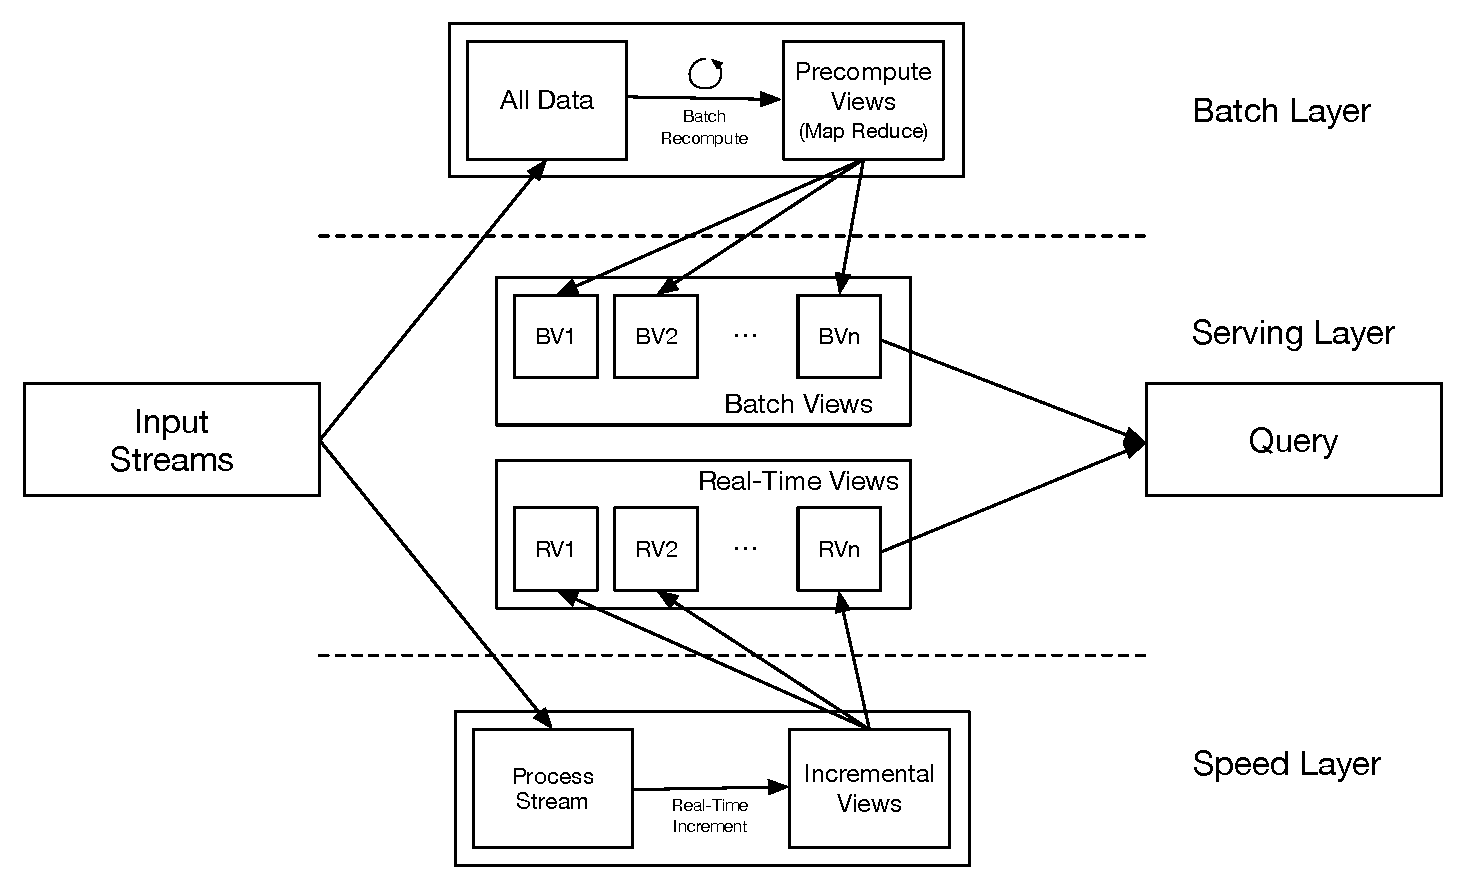
\includegraphics[width=\textwidth]{img/lambda-arch}
    \caption{The $\lambda$ architecture.}
    \label{fig:lambda-arch}
  \end{center}
\end{figure}

In a system implementing a $\lambda$ architecture (see Figure~\ref{fig:lambda-arch}), a separation between the batch processing pipeline (a.k.a. Batch Layer) and the real-time processing pipeline (a.k.a. Real-time Layer) is easily identifiable. This clear separation helps to isolate and localize the complexity of data update. The Serving Layer offers a mechanism to combine Batch Layer results with Real-time Layer results in order to offer the latest information to the user. The three layers are depicted in Figure~\ref{fig:lambda-arch}.
The Batch Layer is in charge of storing the immutable, constantly growing master dataset and of computing views from the stored dataset. 
The computation of the views is a periodic operation, the new data is aggregated once arrived and the views are incrementally computed on the entire dataset every time.
The Batch Layer operations could take hours to be completed, depending on the size of the cluster and of the data.
The Speed Layer compensates the high latency of the Batch Layer. It, normally, computes real-time views on the most fresh data. The views, computed by the Speed Layer, contain only the delta results to supplement the ones computed by the Batch Layer.
The Speed Layer continuously computes real-time views. That views are transient, once the information propagates through the Batch and Serving Layers the corresponding results in the real-time views lost its validity.
The Serving Layer is responsible for merging, indexing and exposing the views in order to make them available for query operations.

In recent years the complexity and the maintenance cost of $\lambda$ architectures were criticized\footnote{\url{https://www.oreilly.com/ideas/questioning-the-lambda-architecture}} and Jay Kreps proposed the $\kappa$ architecture\footnote{\url{http://milinda.pathirage.org/kappa-architecture.com/}}, a stream-only architecture.

\begin{figure}[t]
  \begin{center}
    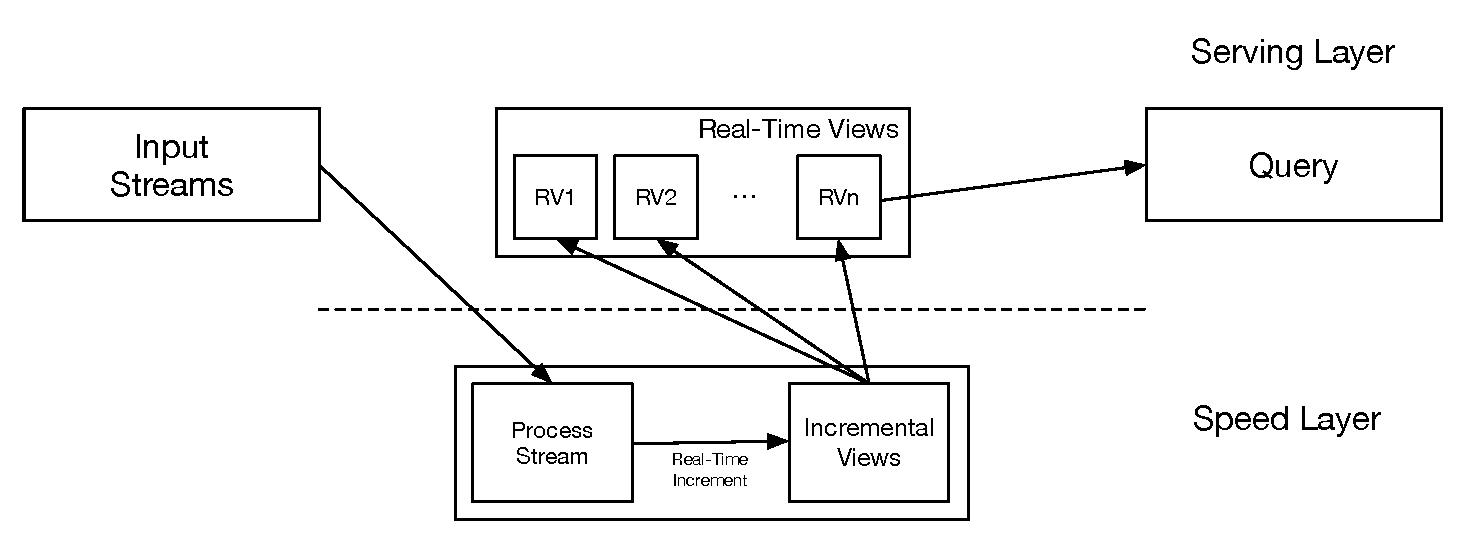
\includegraphics[width=\textwidth]{img/kappa-arch}
    \caption{The $\kappa$ architecture}
    \label{fig:kappa-arch}
  \end{center}
\end{figure}

Figure~\ref{fig:kappa-arch} depicts the main components of the $\kappa$ architecture, that aims at exploiting a single stream processing engine to handle real-time data processing and continuous reprocessing.
In this architecture the Speed Layer are in charge of computing real-time views on the most fresh data from the Input streams. The Real-Time views are incrementally computed when new data enters the system.
The most recent views are available to the Serving Layer for querying operation.
In a system based on a $\kappa$ architecture, the canonical data store is an append-only immutable log.

Both $\kappa$ and $\lambda$ architectures inspired our system presented in Section~\ref{sec:vel-sol} and our Computational Model presented in Chapter~\ref{ch:computational}.

\subsection{Open Source Solutions} \label{sec:vel-sol}
In this section, we present open-source solutions for taming velocity. All the proposed systems represent implementations of a $\lambda$ or a $\kappa$ Architecture. 
We choose to work with open-source software in order to explore and modify the internals to cope with our needs.
The section proposes one vertical scalable system (ESPER) and four different horizontally scalable systems with different characteristics (Kafka, Spark, Hive and Flink).
The proposed solutions inspired our streaming Computational Model proposed in the Chapter~\ref{ch:computational}.

\subsubsection{ESPER \& EPL} \label{sec:esper-epl}
Esper\footnote{\url{http://www.espertech.com/esper/}} is an open-source system for complex event processing (CEP) and streaming analytics. 
Esper exploits in-memory processing to address the requirements of applications that analyze high volume of fast data (between 1,000 to 100k messages per second in input), and must promptly react to events (from a few milliseconds to a few seconds of latency) by applying complex computations (e.g., pattern detection, filter, aggregation, etc.)

The Event Processing Language (EPL) offers SELECT, FROM, WHERE, GROUP BY, HAVING and ORDER BY clauses and is compliant to the SQL-92 standard.
In the EPL logic, streams replace tables as primary source of data and, instead of rows, events become the basic information unit. As for rows in the relational environment, events are composed by data.
EPL allows the definition of windows over stream of data to define a subset of the data to be analyzed. Such windows can be time-based or event-based (see Section~\ref{sec:CQL}) and can be combined applying intersection or union operators. Moreover, EPL provides the concept of named window, a data windows that can be used in multiple statements via the FROM clause, in a join or in a sub-query. 

Together, Esper and EPL, provide a powerful and extendable environment for stream processing and implements the basic concepts of a $\kappa$ Architecture (see Section~\ref{sec:vel-arch}).
Esper is a key components of the C-SPARQL Engine (see Section~\ref{sec:vel-var-solutions}).

\subsubsection{Apache Kafka \& KSQL} \label{sec:kafka}
Apache Kafka \cite{kreps2011kafka} is a distributed message broker with stream processing capabilities. Kafka organizes data into \textit{topics}. Each topic is made up of one or several \textit{partitions}. Each partition is assigned to a node in the Kafka cluster. 

The Kafka APIs are based on the \textit{producer} and \textit{consumer} components. The producer is responsible for transferring data from an external source to a Kafka cluster. Conversely, the consumer is responsible for reading data from a Kafka cluster and sending it to an external sink. By instantiating and using these components, an application can integrate Kafka as its storage solution. Kafka is designed to enable high-throughput applications, and it supports at-least-, at-most-, and exactly-once message delivery.

KSQL\footnote{\url{https://www.confluent.io/product/ksql/}} is a streaming SQL engine for real-time data processing against Apache Kafka. KSQL offers SQL-like language and ensures scalability and fault-tolerancy while enabling commons streaming operations (e.g. window, filter, aggregations, etc).

A system based on Kafka and KSQL enables all the commons operators described in CQL (see Section~\ref{sec:CQL}) and represents an implementation of a $\lambda$~Architecture (see Section~\ref{sec:vel-arch}).
Kafka is a key component of the infrastructure we used to test our work, see Section~\ref{sec:comp-mod-eval-cost}

\subsubsection{Apache Spark} \label{sec:spark}
Apache Spark \cite{zaharia2016apache} is a distributed processing engine which improves the Apache Hadoop~\cite{dean2008mapreduce} cluster computing paradigm for processing massive amounts of data in parallel. The main advantage over Apache Hadoop is that intermediate results can be stored into main memory, thus reducing disk I/O operations.

Spark environment consists of several components, which communicate with each other via the network. The highest level components are the \textit{master} and the \textit{workers}. The master is responsible for coordinating the execution of a Spark application and presenting its results. The workers are responsible for managing the execution of the distributed application code. There can be more than one worker, and each physical machine can host several workers. Both the master and the workers are implemented as separate processes running in the JVM.

Apache Spark is based on the Resilient Distributed Dataset (RDD) abstraction. An RDD represents an immutable dataset distributed over a cluster of machines. Each fragment of the dataset is termed a \textit{partition}. A Spark application consists of a sequence of transformations on a collection of RDDs. During execution, these transformations run in parallel on each partition. When an aggregated result is needed, e.g. COUNT after GROUP BY, Spark performs a shuffle operation by transferring partitions over the network between workers. Each worker spawns several subprocesses known as \textit{executors}. Executors run the distributed application code. The atomic unit of parallel execution is called a \textit{task}. At runtime each task is assigned to an executor.

Spark Streaming~\cite{DBLP:conf/sosp/ZahariaDLHSS13} is an extension of the core Spark API that enables scalable, high-throughput, fault-tolerant and real-time processing of data. 
It offers adapters for various data sources (e.g. Kafka, Flume, etc.).
The key abstraction behind Spark Streaming is the DStream (Discretized Stream), a potentially infinite flow of small batches. DStream are built on RDDs.
Spark Streaming represents an attempt to enable streaming, interactive, and batch queries in a single engine that supports: (i) continuous aggregations, (ii) windowing operations, (iii) stateful stream aggregations, and (iv) stream watermark operations.

Structured Streaming~\cite{DBLP:conf/sigmod/ArmbrustDTYZX0S18} is a new declarative streaming API available starting from Apache Spark 2.0 to support continuous applications. It is a higher-level API than the one offered by Spark Streaming and it is integrated into Dataset and DataFrame API.
Structured Streaming treats all the input data as an unbounded input table, each new items is appended once arrived. The queries see the input as a static table and the system compute the results incrementally.
Structured Streaming represents streams as DataFrames or Datasets with the isStreaming property set to true, therefore, the creation of an application with both stream and batch operations results very simple. A developer has just to describe the query at higher level, with few information about input, output and other details, and the system runs the query incrementally supporting consistency and recovery operations.

We exploited Spark Structured Streaming to create a distributed implementation of our streaming Computational Model presented in the Chapter~\ref{ch:computational}.

\subsubsection{Apache Hive} \label{sec:hive}
Apache Hive~\cite{DBLP:journals/pvldb/ThusooSJSCALWM09} is an open-source data ware-housing solution built on top of Apache Hadoop~\cite{dean2008mapreduce}. It offers a SQL-like declarative language, namely HiveQL, that supports the insertion of custom map-reduce scripts directly into queries.

Hive data is organized into: (i) the Database -- the counterpart of the relational databases --, (ii) the Table -- an abstraction of the classic relational tables, it corresponds to an HDFS directory that contains the serialized data --, (iii) the Partition -- it represents the organization of the data in the sub-directories tree --, (iv) the Bucket -- a division of the data within a partition, a single bucket is represented as a single file.
Hive has a limited support to streaming data. Hive Streaming API allows a system to continuously ingest information in small batches into an existing Hive partition or table. Once the flowing information is committed, it becomes immediately available to all Hive queries.

HiveQL supports primitive data-types within a table, but the underlying IO libraries can be extended to access data in custom formats.
Hive includes a system catalog, the Hive-Metastore. It contains schemas and statistics to be used during the data exploration phases.
HiveQL support a simple window operator\footnote{\url{https://cwiki.apache.org/confluence/display/Hive/LanguageManual+WindowingAndAnalytics}} that can partially simulate the CQL window operator (see Section~\ref{sec:CQL}).  

Hive implements typical batch operator and offers a minimal support for the streaming operations (i.e. window operator). We exploited Hive windows to implement a distributed version of Our streaming Computational Model presented in the Chapter~\ref{ch:computational}.

\subsubsection{Apache Flink}
Apache Flink \cite{DBLP:journals/debu/CarboneKEMHT15} is a distributed platform for streaming data (DataStream API) and batch data (DataSet API). The dataflow engine, the core of the platform, guarantees the fault tolerance during the distributed computations.
Flink's provides an event-at-a-time processing model throw a dataflow of streams and transformations. The DataStream API enables classic stream processing operations (e.g., filters, aggregations, window functions) on bounded or unbounded streams of data, the DataSet API enables transformations (e.g. filters, mapping, joining, grouping) only on finite dataset.

Flink offers a relational abstraction of the data, the Table, that can be created from external data sources or from existing DataStreams and DataSets. The table can be accessed via: (i) the Tables API, a SQL-like expression language that supports relational operators (e.g., selection, aggregation, joins); and via (ii) regular SQL. Both of the access methods offer equivalent functionalities and can be mixed in the programming flow.

Flink can natively manage both stream and batch of data. A system based on it, represents an implementation of a $\lambda$ architecture (see Section~\ref{sec:vel-sol}).

\section{Variety}\label{sec:variety}
In the next sections, we present an overview of the Models, Languages and Methodologies to tame the data variety. After an overview on the main concepts behind RDF, SPARQL and R2RML mapping language, we go through the ontological world.
Gruber in \cite{DBLP:journals/ijmms/Gruber95} define an ontology as "an explicit specification of a conceptualization". A conceptualization is defined as "the objects, the concepts and other entities that are assumed to exist in some area of interest and relationships that hole among them" ~\cite{DBLP:books/daglib/0005829}. An ontology, with its capability to offer a common representation of heterogeneous data, offers a good starting point in facing the variety problem.
The following sections present OWL, an overview of two ontology engineer methodologies (METHONTOLOGY and NEON) and OBDI as an example of integration methods based on ontologies.   
Finally, we present the open source solutions that we exploited during our research work.

\subsection{Models, Languages and Methodologies}

\subsubsection{RDF \& SPARQL}\label{sec:rdf-sparql}
The Resource Description Framework (RDF) is a W3C standard for data interchange on the Web~\cite{cyganiak2014rdf}. 
The main data structure in RDF is the directed labeled graph, made of nodes, which represent the resources and of edges which represent the relations between them. The atomic RDF element is the triple that consists of subject, predicate, and object. We identify with I, B and L respectively the sets of IRIs, blank nodes, and literals. We define an RDF term as an element of the set $I \cup B \cup L$.

\begin{Definition}
(RDF statement and RDF graph). An RDF statement is a triple $(s, p, o) \in (I \cup B) \times (I) \times (I \cup B \cup L)$, while a set of RDF statements is called an RDF graph, which is a directed, labeled graph that represents Web resources.
\end{Definition}

The SPARQL Protocol and RDF Query Language (SPARQL)~\cite{harris2013sparql} is W3C Recommendation and enables data retrieve, data manipulation and query operation on data stored in RDF format.
A SPARQL query typically contains one or more triple patterns called a basic graph pattern, it is similar to an RDF triple except for the possible presence of variables instead of resources.

\begin{Definition}
(Triple pattern and Basic Graph Pattern). A triple pattern $tp$ is a triple $(sp, pp, op)$ such that
\noindent\begin{align*}
(sp, pp, op) \in (I \cup B \cup V ) \times (I \cup V ) \times (I \cup B \cup L\cup V ),
\end{align*}  
where $V$ is the infinite set of variables. 
A basic graph pattern is a set of triple patterns.
Graph patterns in a SPARQL query can include basic graph patterns and other compound expressions defined recursively as:
\begin{enumerate}[nosep]
\item A set of triple patterns is a basic graph pattern;
\item If $P_1$ and $P_2$ are graph patterns, then ($P_1$ AND $P_2$), ($P_1$ OPT $P_2$) and ($P_1$ UNION $P_2$) are graph patterns;
\item If $P$ is a graph pattern and u is a symbol in $I \cup V$, (GRAPH $u$ $P$) and (SERVICE $u$ $P$ ) are graph patterns;
\item If $P$ is a graph pattern and $R$ is a SPARQL built-in condition, then ($P$ FILTER $R$) is a graph pattern.
\end{enumerate}
\end{Definition}

A SPARQL built-in condition consists of the elements of the set
$(I\cup L \cup V)$ and constants, logical connectives $(\neg, \vee, \wedge)$, the binary equality symbol $(=)$, ordering symbols
$(<,\leq,\geq,>)$, and unary predicates such as $bound$,
$isBlank$, $isIRI$.

To introduce the evaluation semantics of a SPARQL query, we define solution mapping as detailed in~\cite{DBLP:journals/tods/PerezAG09,harris2013sparql}.

\begin{Definition}
(Solution mappings). A solution mapping $\mu$ is a partial function $\mu \colon V \rightarrow I \cup B \cup L$. It maps a set of variables to a set of RDF terms. 
A mapping has a domain $dom(\mu)$ which is the subset of V over which it is defined. We denote as $\mu(x)$ the RDF term resulting by applying the solution mapping to variable $x$. We denote as $\omega$ a multiset of solution mappings, and as $\psi$ a sequence of solution mappings. 
Typical relational algebraic operators can be applied to multiset of solution mappings:
\begin{itemize}[label={}, nosep]
\item $\Omega_1\Join\Omega_2 = \{\mu_1 \cup \mu_2 | \mu_1 \in \Omega_1 \wedge \mu_2 \in \Omega_2 \wedge \mu_1 \sim \mu_2\}$
\item $\Omega_1 \cup \Omega_2 = \{\mu| \mu_1 \in \Omega_1 \vee \mu_2 \in \Omega_2\}$
\item $\Omega_1 \backslash \Omega_2 = \{\mu| \mu \in \Omega_1 \wedge \nexists \mu_1 \in \Omega_2 \colon \mu \sim \mu_1\}$
\item $\Omega_1\leftouterjoin\Omega_2 = (\Omega_1\Join\Omega_2) \cup (\Omega_1 \backslash \Omega_2)$
\end{itemize}  
\end{Definition}

RDF datasets is a collections of one or more RDF graphs and represents the format of input data.
\begin{Definition}
(RDF dataset). An RDF dataset DS is a set: 
\noindent\begin{align*}
DS = {G0, (u1, G1), (u2, G2), ...(un, Gn)}
\end{align*}
where G0 and Gi are RDF graphs, and each corresponding ui is a distinct IRI. G0 is called the default graph, while the others are called named graphs. During the evaluation of a query, the graph from the dataset used for matching the graph pattern is called active graph. Multiple graphs can become active during the evaluation, but only one at time.
\end{Definition}

SPARQL defines four query forms: SELECT -- which produces a result of variable bindings matching the graph pattern --, CONSTRUCT, which produces a new RDF graph with the query solutions --, ASK -- which produces a boolean value that is true if at least a solution exists --, and DESCRIBE -- which produces an RDF description of resources in the solution.
A query can also contain solution modifiers (e.g., LIMIT, DISTINCT, ORDER BY) that are applied after pattern matching.
A SPARQL query \cite{DBLP:journals/tods/PerezAG09} can be defined as:

\begin{Definition}
(SPARQL Query). A SPARQL query is defined as a tuple (E, DS, QF), where E is a SPARQL algebraic expression, DS is an RDF dataset, and QF is a query form.
\end{Definition}

A query solution is a bag of solution mappings that assign RDF triples to variables of the query.
The evaluation semantics of a SPARQL query algebraic expression w.r.t. an RDF dataset is defined for every operator of the algebra, and it is expressed through an evaluation function.

\begin{Definition}
(SPARQL evaluation semantics). The SPARQL evaluation semantics of an algebraic expression E is denoted as ED(G), where DS(G) is the dataset DS with active graph G.
\end{Definition}

RDF and SPARQL represent a fundamental concepts in the data variety management, both in static and streaming environment (see Section~\ref{sec:vel-var}).

\subsubsection{R2RML}
The RDB to RDF mapping language\footnote{\url{http://www.w3.org/TR/r2rml/}} (R2RML) is a language to create custom mappings to transform relational data into RDF.
R2RML mappings file presents itself as an RDF graphs and, unlike Direct Mapping\footnote{\url{https://www.w3.org/TR/rdb-direct-mapping/}} (DM), allows user to define highly customized views over relational data sources. The R2RML conceptual mapping is tailored to a specific database schema and target vocabulary (i.e., the input database must conform to the presented schema) and produces an RDF dataset (see Section~\ref{sec:rdf-sparql}) that conforms to the target vocabulary. The R2RML processors can work as a virtual access layer to the relational data or can materialize the output data.

\begin{figure}[t]
  \begin{center}
    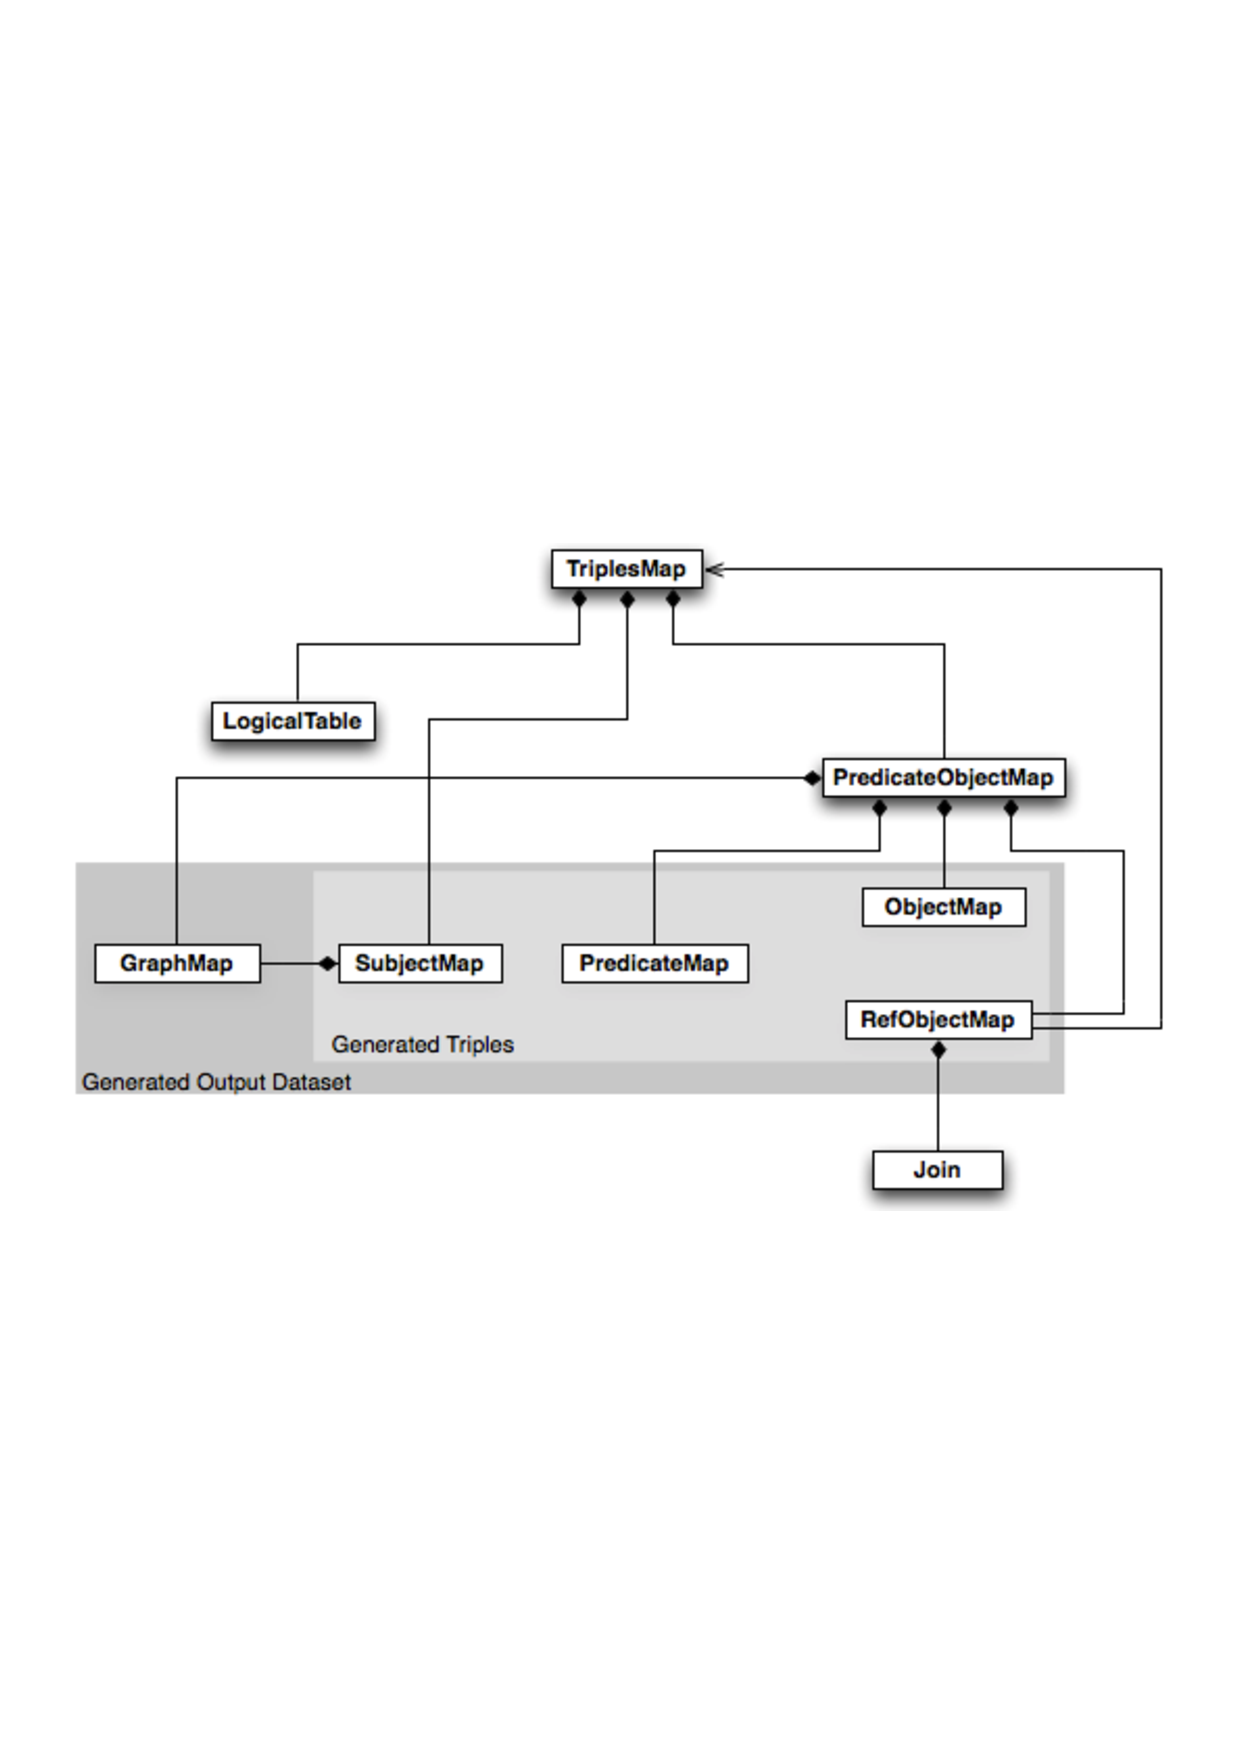
\includegraphics[width=0.8\textwidth]{img/R2RML}
    \caption{R2RML mapping process (source: https://www.w3.org/TR/r2rml).}
    \label{fig:r2rml}
  \end{center}
\end{figure}

Figure~\ref{fig:r2rml} depicts the overview of the mapping process.
R2RML mapping accesses to the relational input data through logical tables. A logical table can be a base table in the input database, a view or a valid SQL query (R2RML view).
Each logical table is then mapped to RDF using a triple map, a set of rules that allows the system to transform each row in the logical table into one or more RDF triples. The rules are composed by a subject map that creates the subject for all the triples generated by a single row and by multiple predicate-object maps that consist of predicate maps and object maps.

\subsubsection{OWL} \label{sec:owl}
The Web Ontology Language (OWL)\footnote{\url{https://www.w3.org/TR/owl-features/}} is a W3C Semantic Web language designed for creating ontologies.
OWL is part of the W3C's Semantic Web technology stack. It is a computational logic-based declarative language  characterized by formal semantics.
The knowledge expressed in OWL can be reasoned to verify the consistency of that knowledge or to make implicit knowledge explicit.
The fundamental notions exploited by OWL to represent knowledge are: (i) the Axioms -- the basic statement of an ontology --, (ii) the Entities -- the representation of a real world object --, and (iii) the Expressions -- a combination of entities to describe a complex object.

The three concepts presented above allow OWL to create a human-like knowledge representation with the concept of consequence. When a statement is a consequence of another statement, it is true whenever the other statements are. In OWL, a set of statements \textit{S} entails a statement \textit{s} if in any state of affairs wherein all statements from \textit{S} are true, also \textit{s} is true. A set of statements may be consistent (there is a possible state in which all the statements in the set are jointly true) or inconsistent (there is no such state). The formal semantics of OWL specifies for which condition a particular set of OWL statements is true.

The W3C-endorsed OWL specification includes the definition of three variants of OWL: OWL Lite, OWL DL and OWL Full, presented in order of expressiveness.
OWL2\footnote{\url{https://www.w3.org/TR/owl2-overview/}} represents the latest specification of the  Web Ontology Language. It is dated to 2009 and introduces three additional profiles: OWL2EL, a fragment with polynomial time reasoning complexity; OWL2QL, a language to enable easier access and query to data stored in databases; and OWL2RL, a rule subset of OWL2.

The Conceptual Model presented in the Chapter \ref{ch:conceptual} is formalized with OWL2.

\subsubsection{Ontology Engineering}\label{sec:onto-eng}
We report a briefly overview of METHONTOLOGY, an ontology development methodology we exploited in the definition of the Conceptual Model presented in Chapter~\ref{ch:conceptual}, and NeOn, an evolution of METHONTOLOGY, that supports the reuse of already available ontologies.

\textbf{METHONTOLOGY}~\cite{fernandez1997methontology} is a methodology for creating ontologies from scratch, by reusing other ontologies or by re-engineering them. The framework enables the construction of ontologies at the "knowledge level". 

\begin{figure}[h]
  \begin{center}
    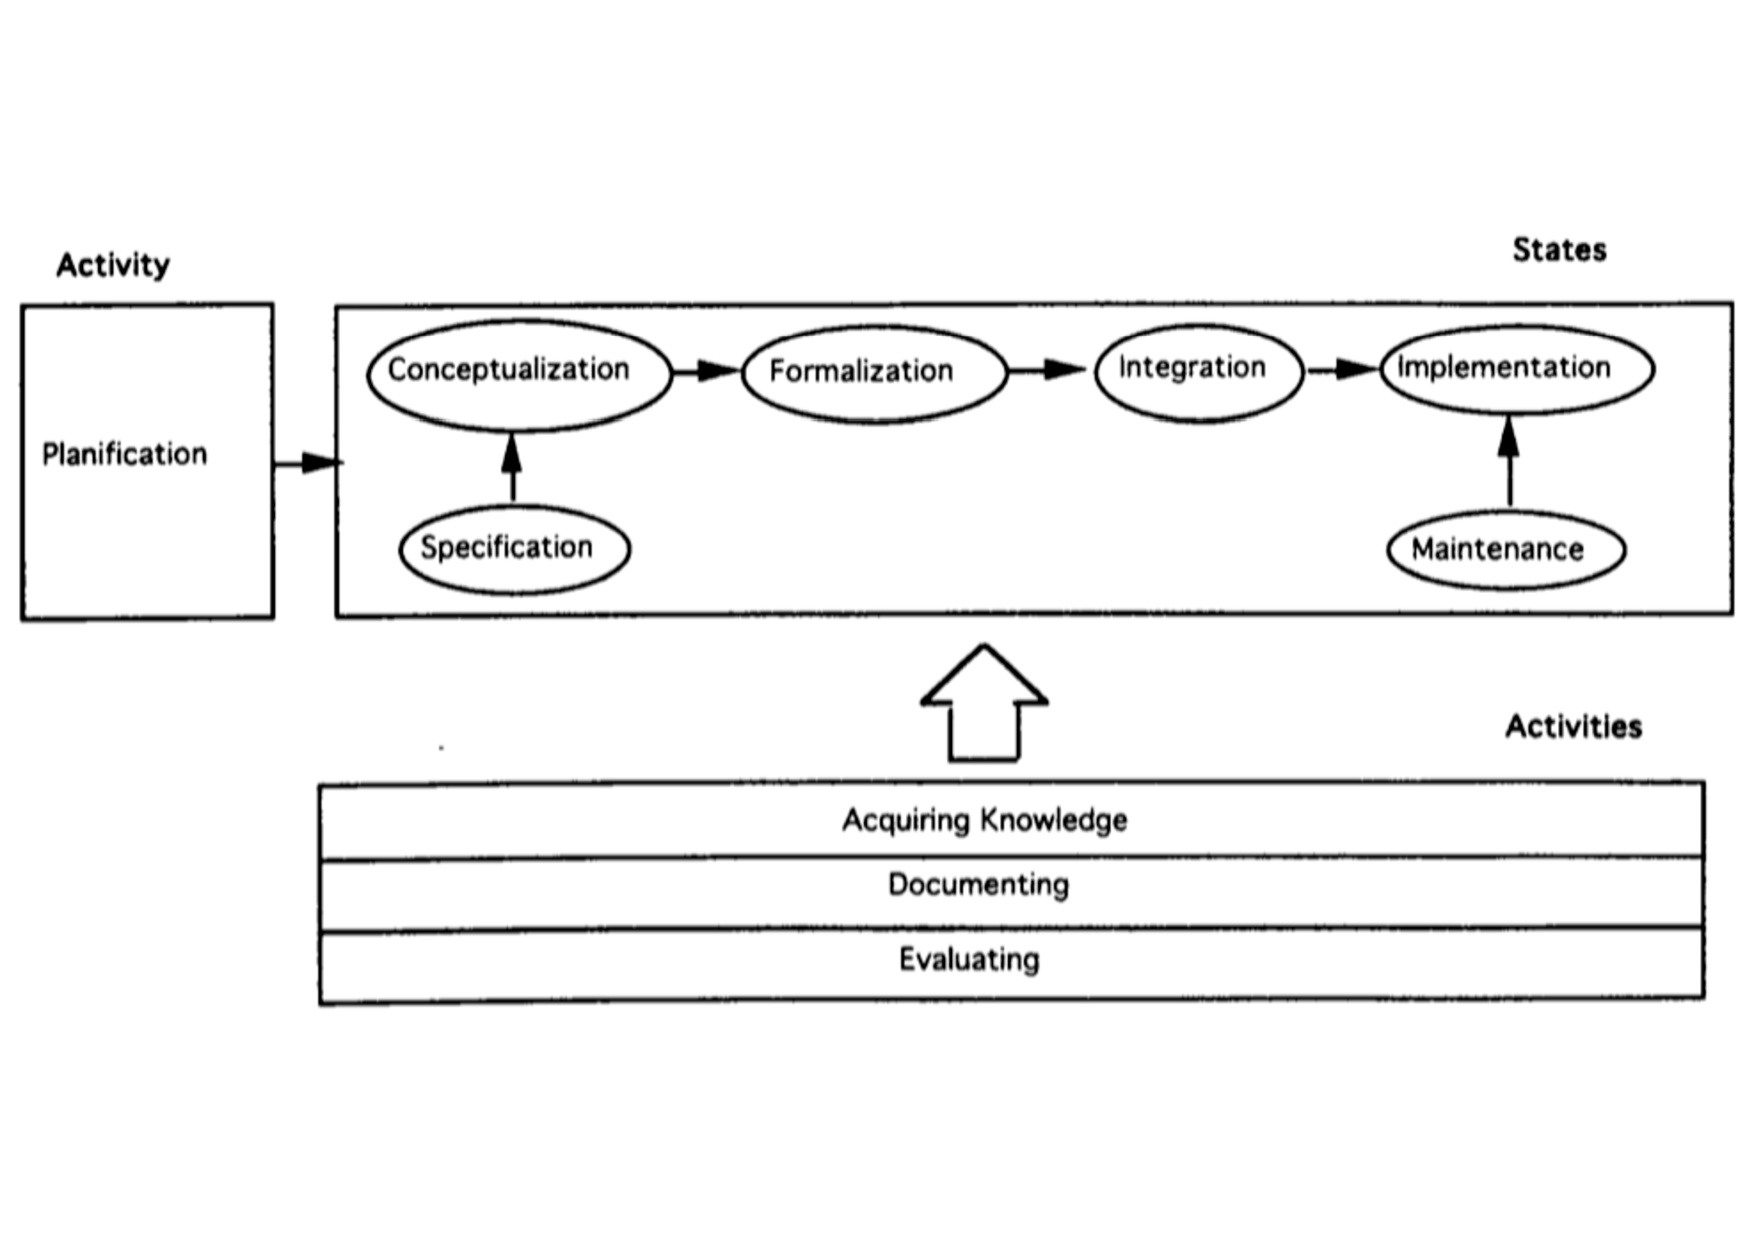
\includegraphics[width=0.8\textwidth]{img/methontology}
    \caption{Ontology lifecycle (source~\cite{fernandez1997methontology}).}
    \label{fig:methontology}
  \end{center}
\end{figure}

It includes: (i) the formal identification of the development process and its phases (i.e., scheduling, control, quality assurance, specification, knowledge acquisition, conceptualization, integration, formalization, implementation, evaluation, maintenance, documentation and configuration management); (ii) an evolving prototypes based lifecycle (see Figure~\ref{fig:methontology}) that identifies the phases the ontology passes during its lifetime and the interdependencies with the lifecycle of the connected ontologies; (iii) the specific techniques to perform each activity, the output of each phases and the evaluation methods.

The \textbf{NeOn}~\cite{DBLP:phd/dnb/Suarez-Figueroa12} methodology encourage the reuse of other ontologies as well as of non-ontological resources during the engineering process. The framework provides strong guidelines for the execution of the development activities (e.g., the usage of ontology design patterns). 

\subsubsection{OBDI \& OBDA}\label{sec:obdi-obda}
The data integration problem consists of combining data from heterogeneous sources, and offering the user a unified view of the information. Due to the growing number of data sources (e.g., smartphones, sensors, etc), the  problem of designing data integration systems are becoming more and more important in the real-world.
Moreover, companies are shifting from centralized and self-contained way to manage their data (i.e., a central database or a data warehouse) to a distributed, interactive and multi-source world where the information becomes the exchange good. The volume and the heterogeneity of the data are constantly growing and companies are now focusing on finding the right information.
Most of the available sources is characterized by syntactic, structural and semantic heterogeneities.

In a generic data integration system~\cite{LenzeriniOBDI}, the sources contain the real data, while a global schema offers an integrated and reconciled overview of such sources. Modeling the relation (namely, the mapping) between the sources and the global schema represents an important aspects of the data integration process.
The data integration issue have been faced following three different approaches: (i) the Global-As-View (GAV) approach -- the most used form of mappings, where the data schema is expressed in terms of the data sources --, (ii) the Local-As-View (LAV) approach -- where the data schema is specified independently from the sources --, and a hybrid approach (GLAV) -- the most general form of mapping.
Independently from the approach, in a data integration system, the query process requires a reformulation step where the query over the global schema is reformulated in terms of a set of queries over the sources.

In several domains, such as Enterprise Application Integration, in the Semantic Web and, in particular, in the data integration~\cite{LenzeriniOBDI}, ontologies are considered as the ideal formal tool to provide a common conceptualization of the domain, and Description Logics (DLs) are widely considered appropriate for expressing ontologies. DLs are also at the basis of the OWL Language (see Section~\ref{sec:owl}).

Consequently, an Ontology-Based Data Integration (OBDI) system consists of three main components: (i) an ontology -- the formal description of the considered domain --, (ii) a set of data sources -- the repositories where data are stored --, and (iii) the mapping -- a specification of the correspondences between the data and the ontology elements. Such system allows users to access the data using the ontology components as a predicates. 
Differently from the traditional data integration, OBDI system offers a semantically rich description of the relevant concepts in the domain of interest and of the relationships between such concepts, in addition to a separation between the conceptual level (presented to the client through the ontology),
and the logical/physical level of the information system (the one stored in the sources).

Intuitively, in the simplest technique for enabling query answering, the system first retrieves the concepts and the roles instances from the data sources through the mapping and then, exploiting the ontology axioms, it "expands" such a set of (stated and inferred) instances deriving and materializing all the logically entailed concepts and roles assertions. 
In this way, the queries can be evaluated on the complete set of instances. Unfortunately, the set of entailed instance assertions may be infinite and, consequently, such a techniques is not feasible. 

Since 2000s, Ontology-Based Data Access (OBDA)~\cite{DBLP:journals/jods/PoggiLCGLR08} has become a popular approach to enable users to access data sources through an ontology.
Moreover, a GAV approach based on a data model expressed in OWL 2 QL (based on the DL-Lite family of description logics), ensures the effectiveness of query answering operation with LOGSPACE complexity (more precisely, AC\textsuperscript{0}).

In a classic OBDA framework, query rewriting starts from the computation of the perfect rewriting in order to enable the query evaluation on the data sources. The creation of the rewriting can be modularized into a first phase of of query rewriting related to the ontology and in a second phase of query rewriting related to the mapping.

During our research work we exploited OBDI and OBDA techniques in many applications (see Chapter~\ref{ch:case-studies}) using our Conceptual Model presented in Chapter~\ref{ch:conceptual} as the ontology to mediate between the user queries and the data.

\subsection{Open Source Solutions} \label{sec:var-solutions}
In this section, we present the solutions we used over the years in our research work. As usual in this research, we have privileged open source solution in order to access and exploits the internals.

We start from Jena and Sesame, frameworks to manage RDF data and to build Semantic Web applications.
\textbf{Apache Jena}\footnote{\url{https://jena.apache.org/}} is written in Java.
The main data structure in Jena is the Model, an abstract representation of an RDF graph.
A model can be accessed and queried via SPARQL and its source can be external file, databases, URLs or a combination of them.
Jena offers different components to support the creation of application, it provides the TDB, an RDF database that supports SPARQL 1.1 query, and Fuseki, a database server that support the access via the standard SPARQL protocols\footnote{\url{http://www.w3.org/TR/sparql11-protocol/}}. Jena is a core component of the C-SPARQL Engine (see Section~\ref{sec:vel-var-solutions}).

\textbf{Sesame}~\cite{DBLP:conf/semweb/BroekstraKH02} is an open-source framework for storing, querying and analyzing RDF data. It also offers support for RDFS inferencing and querying.
Sesame implements an in-memory/on-disk triplestore and offers a Servlet packages to manage and access the stored data on a permanent server. 
Sesame supports concurrency control, export of RDF and RDFS information and a query engine for RQL, SPARQL and SeRQL.
In May 2016, Sesame officially forked into an Eclipse project called RDF4J\footnote{\url{http://rdf4j.org}} that provides functionality for efficient and scalable storage, querying, and reasoning with RDF data, and a vendor-neutral access API for RDF databases.

To explore the basic reasoning techniques we worked with Hermit and RDFox. 
\textbf{HermiT}~\cite{DBLP:conf/owled/ShearerMH08} is a Description Logic reasoner based on a "hypertableau" calculus techniques, an innovative and efficient reasoning algorithm. It also incorporates the "anywhere blocking" strategy, which limits the sizes of constructed models.
HermiT uses direct semantics and is conformant to all OWL 2 tests for direct semantics reasoners.
\textbf{RDFox}~\cite{DBLP:conf/semweb/NenovPMHWB15} is a main-memory, scalable, centralized datalog engine. It supports materialization-based parallel reasoning, SPARQL query answering and implements Backward/Forward algorithm proposed in~\cite{DBLP:conf/aaai/MotikNPH15a}.
The innovative intuition is the combination of backward and forward reasoning to limit the recomputation performed by the traditional DRed~\cite{DBLP:journals/jods/VolzSM05}.

As OBDA framework, we used \textbf{OnTop}~\cite{DBLP:journals/semweb/CalvaneseCKKLRR17}, an open-source Ontology-Based Data Access (OBDA) system that offers a solid theoretical base, a virtual OBDA approach implemented with query rewriting technique, its compliance to W3C recommendations and its support for all major relational databases.

\begin{figure}[t]
  \begin{center}
    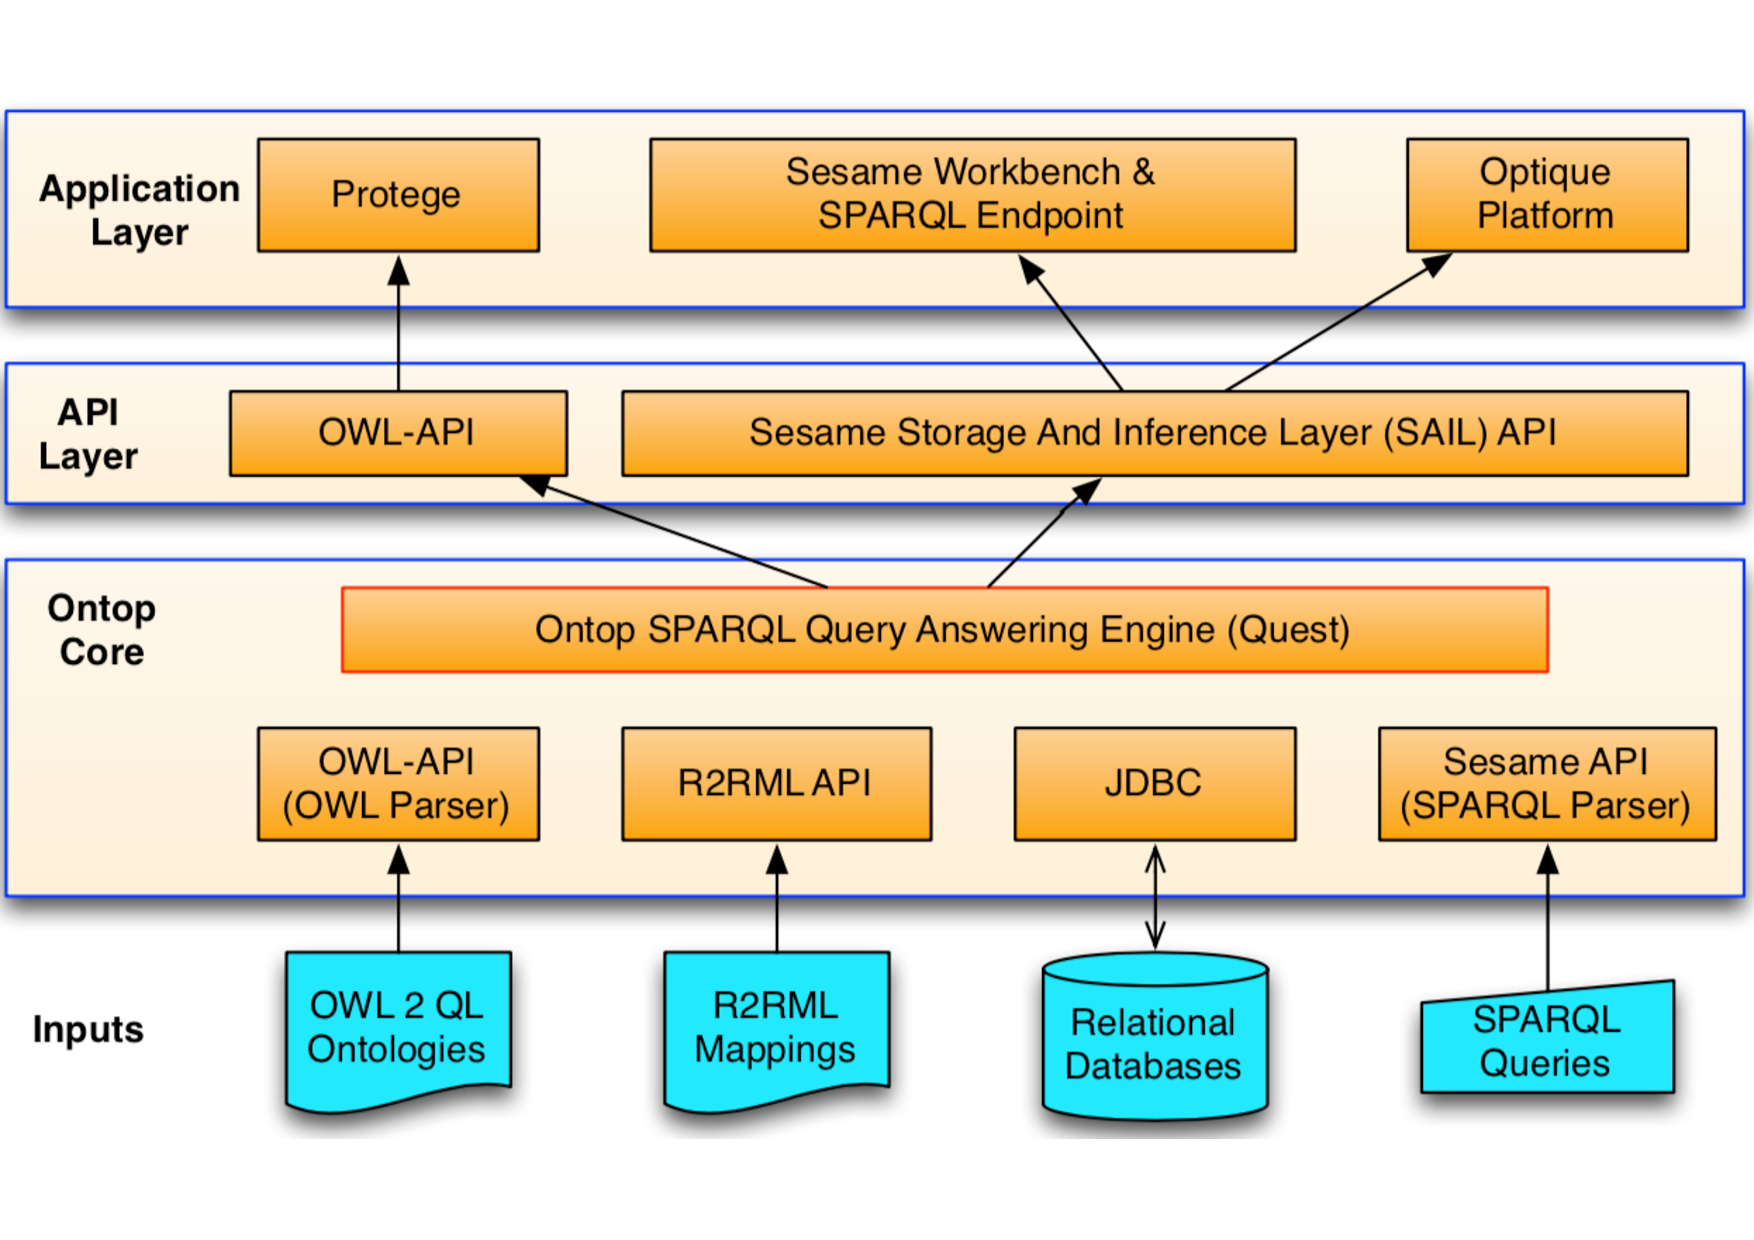
\includegraphics[width=0.8\textwidth]{img/ontop}\\
    \caption{Architecture of the Ontop system (Source \cite{DBLP:journals/semweb/CalvaneseCKKLRR17}).}
    \label{fig:ontop}
  \end{center}
\end{figure}

Figure \ref{fig:ontop} presents the four levels of a system based on Ontop: (i) the input, such as queries, database, ontology and mapping; (ii) the Ontop core needed to rewrite SPARQL queries SQL queries; (iii) the API for accessing system services; and (iv) the applications for the end-user to execute SPQARL queries over relational data.

\section{Velocity and Variety}\label{sec:vel-var}
In the next sections, we present the solution to manage the data variety in a streaming fashion. We start from the formal definition of the concepts behind Stream Reasoning and RDF Stream Processing (RSP). We present RSP-QL, an attempt to unify the different RSP query languages developed over the years by the RSP community and, finally, we present an overview of the currently available solutions.

\subsection{Models and Languages}
\subsubsection{Stream Reasoning \& RDF Stream Processing}\label{sec:sr-rsp}
In 2009, Della Valle et al. \cite{della2009s} proposed to start to investigate on how to represent, manage, and reason on heterogeneous continuously flowing data in the presence of expressive domain models.

In a scenario, where an ontology offers a conceptual view over autonomous data sources, a reasoner can play a key role in finding answers that are not syntactically present in the data sources, but are derivable from the data and the ontology (see Section~\ref{sec:obdi-obda} on OBDI and OBDA).
RDF (see Section~\ref{sec:rdf-sparql}) represent the dominant data model in the field of reasoning for data integration and RDF streaming languages (see Section~\ref{sec:vel-var-solutions}) bridge the gap between stream processing and OBDI. 
Reasoning in a streaming fashion looks conceptually simple, but it is hard to be efficiently performed. Della Valle et al. \cite{DBLP:conf/fis/ValleCBBC08} showed how continuous DL reasoning can be reduced to periodic repetition of reasoning over a windowed ontology stream.
Barbieri et al. \cite{DBLP:conf/esws/BarbieriBCVG10} presented an optimization of DRed algorithm when deletion becomes predictable. In parallel Komazec et al. \cite{DBLP:conf/debs/KomazecCF12} implemented an extension of the RETE algorithm, Ren at al. \cite{DBLP:conf/cikm/RenP11} approached the problem via truth maintenance systems and Motik et al. \cite{DBLP:conf/aaai/MotikNPH15a} represents the state of the art in this research field.
Still along this DL-centric line, more recently, Calbimonte et al. \cite{DBLP:conf/semweb/CalbimonteCG10} exploited OBDA principles by rewriting continuous ontological queries to a stream processing system. In parallel to this line, at the beginning of 2000s Heintz et al.~\cite{DBLP:journals/jifs/HeintzD04} proposes a first approach to middleware for knowledge processing and in~\cite{DBLP:phd/basesearch/Heintz09} an implementation of this approach. More recently, De Leng et al. \cite{DBLP:conf/aaai/LengH16} proposed logic-based spatio-temporal stream reasoning focusing on run-time verification to guarantee the safety of autonomous systems and Anicic et al. \cite{DBLP:journals/semweb/AnicicRFS12} developed a system that processes in logic programming both stream reasoning and complex event processing.

RDF Stream Processing (RSP) represents the sub-area of stream reasoning that concentrates on the Semantic Web~\cite{DBLP:conf/debs/ValleDM16}.

In this section, we introduce the concept of RDF data item and, consequently, Timestamped RDF data item.
The RDF data item represents the minimal informative unit in the RDF stream. It is a generic concept and the existing RSP implementations (see Section~\ref{sec:vel-var-solutions}) consider it in two different ways: RDF statements and RDF graphs, as defined in Section~\ref{sec:rdf-sparql}.
In the most intuitive case a RDF stream is composed of RDF statements~\cite{DBLP:conf/fis/ValleCBBC08}.
Due to the limited amount of information carried by a single statement, in order to ease the task of model real world use case, in 2010 Barbieri et al.~\cite{DBLP:conf/www/BarbieriV10} proposes to use the RDF graphs. In 2013 we were the first to implement this concept in~\cite{DBLP:conf/semweb/BalduiniVDTPC13}.

The definition of a Timestamped RDF data item can be formalized as:

\begin{Definition}
(Timestamped RDF data item) A timestamped RDF data items is a pair (d,t), where d is an RDF graph and $t \in Ti$ is a time instant. 
\end{Definition}

Once defined the possible nature of the RDF data item, we can now define a RDF stream.
\begin{Definition}
(RDF stream) An RDF stream S is an unbounded sequence of timestamped RDF data items in non-decreasing time order:
\noindent\begin{align*}
S = ((d_1, t_1), (d_2, t_2), ..., (d_{n-1}, t_{n-1}), (d_n, t_n), ...)
\end{align*}  
where, for every $i > 0, d_i$ is a timestamped RDF item and $t_i <= t_{i+1}$.
\end{Definition}

A time-varying RDF graph capture the evolution of graph content over time, contrariwise, instantaneous graph represents the content of the graph at a fixed time instant

\begin{Definition}
(Time-varying Graph) A time-varying graph G is a function that relates time instants $t \in Ti$ to RDF graphs:
\noindent\begin{align*}
G : T \rightarrow {g | g\, is\, an\, RDF\, graph}
\end{align*}
\end{Definition}

\begin{Definition}
An instantaneous RDF graph $G(t)$ is the RDF graph identified by the time-varying graph G at the given time instant t.
\end{Definition}

\begin{figure}[h]
  \begin{center}
    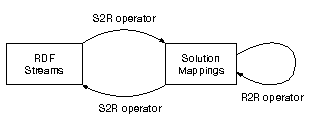
\includegraphics[width=.65\textwidth]{img/cql-rdf-model}\\
    \caption{The CQL processing model adapted for RSP}
    \label{fig:cql-rdf-model}
  \end{center}
\end{figure}

The RDF stream processing model is depicted in Figure~\ref{fig:cql-rdf-model}. It is directly derived from the CQL one (see Section~\ref{sec:CQL}). The stream and the relation concepts are mapped to RDF streams and to set of mappings (using the SPARQL algebra terminology), respectively. To highlight the similarity of the RSP operators \cite{DBLP:journals/ijswis/DellAglioVCC14} to the CQL ones, the same names (\textbf{S2R}, \textbf{R2R} and \textbf{R2S}) are used to indicate the stream-to-relation, relation-to-relation and relation-to-stream operators. 

The concepts described in this section are all implemented in our Streaming Linked Data (SLD) framework (see Section~\ref{sec:sld}) and inspired the definition of our generic streaming Computational Model presented in Chapter~\ref{ch:computational}. 

\subsubsection{RSP-QL} \label{sec:rsp-ql}
%citare cosa prende da SECRET e da CQL
RDF Stream Processor Query Language (RSP-QL) \cite{DBLP:journals/ijswis/DellAglioVCC14} is an extension of SPARQL created to unify existing RSP query languages (i.e, C-SPARQL~\cite{DBLP:journals/ijsc/BarbieriBCVG10}, CQELS~\cite{DBLP:conf/semweb/PhuocDPH11} and SPARQL\textsubscript{stream}~\cite{DBLP:journals/semweb/AnicicRFS12}).
RSP-QL enables user to register continuous queries. The queries are registered once over streams of data and continuously evaluated. Due to the continuous evaluation semantic, a query produces multiple results over time and the instantaneous answer is a composition of the results of each iteration.
RSP-QL is designed following two main requirements: (i) every evaluation of a query over input data produces a unique solution, (ii) RSP-QL, inspired by SECRET(see Section~\ref{sec:secret}), captures the operational semantics of C-SPARQL engine, CQELS and Morph\textsubscript{stream} (see Section~\ref{sec:vel-var-solutions}).
RSP-QL implements the basic concepts of the extensions of SPARQL concepts presented in the Section~\ref{sec:rdf-sparql}.
We start presenting the core concept of the RSP-QL language, the RSP-QL query.

\begin{Definition}
(RSP-QL query) RSP-QL query Q is defined by the tuple (SE,SDS,ET,QF) where
\begin{itemize}
\item SE is an RSP-QL algebraic expression
\item SDS is an RSP-QL dataset
\item ET is the sequence of time instants on which the evaluation occurs
\item QF is the Query Form
\end{itemize}
\end{Definition}

The presence of the time dimension calls for a new notion of RDF dataset, the input data of the RSP-QL query. 

\begin{Definition}
(RSP-QL dataset) An RSP-QL dataset SDS is a set composed by an (optional) default graph, n $(n \geq 0)$ named graphs and m $(m \geq 0)$ named time-varying graphs obtained by the application of time-based sliding windows over $o \leq m$ streams:
\noindent\begin{align*}
SDS =\{G_0, (u_1,G_1), ..., (u_n,G_n),\\
(w_1, W_1(S_1)), ... , (w_j , W_j(S_1)), \\
(w_{j+1}, W_{j+1}(S_2)), ..., (w_k, W_k(S_2)), ..., \\ (w_l,W_l(S_o)), ..., (w_m, W_m(S_o))\}
\end{align*}  
with:
\begin{itemize}
\item $G_0$ is the default time-varying graph
\item $u_p,w_q$ are IRIs $(u_p,w_q \in \mathbb{I})$ for each $p \in [1,n]$ and $q \in [1,m]$
\item $(u_p,G_p)$ identifies a time-varying named
graph, for each $p \in [1, n]$
\item $(w_q , W_q (S_r))$ identifies a named time-based sliding window over an RDF stream, for each $q \in [1, m]$ and $r \in [1, o]$
\end{itemize}
\end{Definition}

In a continuous environment a definition o a time-varying sequence of solution mappings is needed.

\begin{Definition}
(Time-varying sequence of solution mappings)
A time-varying sequence of solution mappings $\psi$ maps time instants $t \in Ti$ to the set of solution mapping sequences:
\noindent\begin{align*}
\psi : T \rightarrow \{\Psi | \psi\, is\, a\, sequence\, of\, solution\, mappings\}
\end{align*}  
\end{Definition}

The RSP-QL evaluation semantic is an evolution of SPARQL evaluation semantic defined taking into account the time dimension.

\begin{Definition}
(RSP-QL evaluation semantic)
Given an RSP-QL dataset SDS, an algebraic expression SE and an evaluation time instant t, we define
\noindent\begin{align*}
eval(SDS(G), SE, t)
\end{align*}  
as the evaluation of SE at time t with respect to the RSP-QL dataset SDS having active time-varying graph G.
\end{Definition}

\subsection{Open Source Solutions} \label{sec:vel-var-solutions}
In the next sections, we present the principal solutions proposed by the Semantic Web community for taming velocity for heterogeneous data. 
In particular, we present vertical RDF Stream Processors developed before the definition of RSP-QL with their own query languages and a couple of distributed implementations. The proposed solution inspired the streaming Computational Model presented in the Chapter~\ref{ch:computational}.

\paragraph{C-SPARQL Engine}
Continuous SPARQL (C-SPARQL)~\cite{DBLP:journals/ijsc/BarbieriBCVG10} is a language to express continuous queries over flowing data in RDF format. It extends SPARQL 1.1 by defining Data Stream Processing operators, including the possibility of defining window over streams of data.
The C-SPARQL engine\footnote{\url{http://streamreasoning.org/resources/c-sparql}} is an open-source software that exploits the C-SPARQL language to enable the registration of continuous queries to be executed over RDF streams.
Its core is based on two sub-components: Esper (see Section~\ref{sec:esper-epl}) and Jena (see~Section~\ref{sec:var-solutions}) . The former is responsible of executing continuous 
operations on the stream, e.g. sliding window to produce RDF graph. The latter periodically executes standard SPARQL query on the RDF stream fragments to produce continuous results.

\paragraph{CQELS}
CQELS-QL~\cite{DBLP:conf/semweb/PhuocDPH11} is a declarative query language that extends SPARQL 1.1 grammar with operators to deal with streaming data. Continuous Query Evaluation over Linked Streams (CQELS) interpret queries in CQELS-QL and, differently from C-SPARQL, supports only the Istream relation-to-stream operator (see Section~\ref{sec:CQL}).
CQELS offers a flexible framework for the query operations with a dynamic adapting processors that continuously reorders operators to improve query execution in terms of delay and complexity.
It natively implements the query operators in order to limit the overhead and the limitations related to the usage of other engines (e.g. C-SPARQL engine relies on Esper and Jena).

\paragraph{Morph\textsubscript{stream}}
SPARQL\textsubscript{stream}~\cite{DBLP:conf/semweb/CalbimonteCG10} extends SPARQL to support all the stream operators (e.g. sliding window).
SPARQL\textsubscript{stream} is implemented in Morph\textsubscript{stream} engine that exploits Ontology-Based Data Access techniques~\cite{DBLP:journals/ijswis/CalbimonteJCA12}.
Morph\textsubscript{stream} execution is based on R2RML\footnote{\url{https://www.w3.org/TR/r2rml/}} mappings between ontologies and data streams.
The queries are first rewritten in a relational algebra expression with time window extension and then translated in the Data Stream Processing target language.

\paragraph{INSTANS}
Incremental eNgine for STANding Sparql (INSTANS) \cite{DBLP:conf/semweb/RinneNT12} enables users to create a flow of multiple SPARQL 1.1 queries that represents a single task. The engine is in charge of continuously evaluates the incoming data and store intermediate results. INSTANS approaches RDF stream processing from a different perspective and does not require a continuous extensions to RDF or SPARQL.

\paragraph{ETALIS and EP-SPARQL}
Event TrAnsaction Logic Inference System (ETALIS) \cite{DBLP:journals/semweb/AnicicRFS12} is an RDF stream processing engine that takes in account two time-stamps during the data processing.
It is a pluggable system that can use multiple prolog engines.
An internal ETALIS task can be specified using two different languages, Event Processing SPARQL (EP-SPARQL) and ETALIS Language for Events (ELE). Both of them allow users to derive complex events through deductive prolog rules. 
The engine supplies the results as soon as they are available and supports three different policies during the execution of the task: (i) unrestricted, all the input items are used for matching the declared patterns; (ii) chronological, the earliest matchable input are selected for matching the event patterns, the next evaluations will ignore the already selected data; (iii) recent, the latest matchable input are selected for matching the event patterns, as for chronological policy, they are then ignored.

\paragraph{CQELS Cloud}
CQELS Cloud~\cite{DBLP:conf/semweb/PhuocQVH13} presents an elastic and distributed environment that exploits an extension of CQELS to enable a network of processing nodes to parallelize tasks.
The input of the CQELS Cloud execution model is a set of CQELS-QL queries to be executed against a set of RDF input streams and the output is a set of output streams (in RDF or relational format).
The input queries are compiled to produce a logical query network that defines the algebras for each input stream. The logical query network is, then, mapped on a processing network made of processing nodes, namely the Operator Containers (OCs). The tasks are distributed among the OCs by the Global Scheduler.

\begin{figure}[h]
\begin{center}
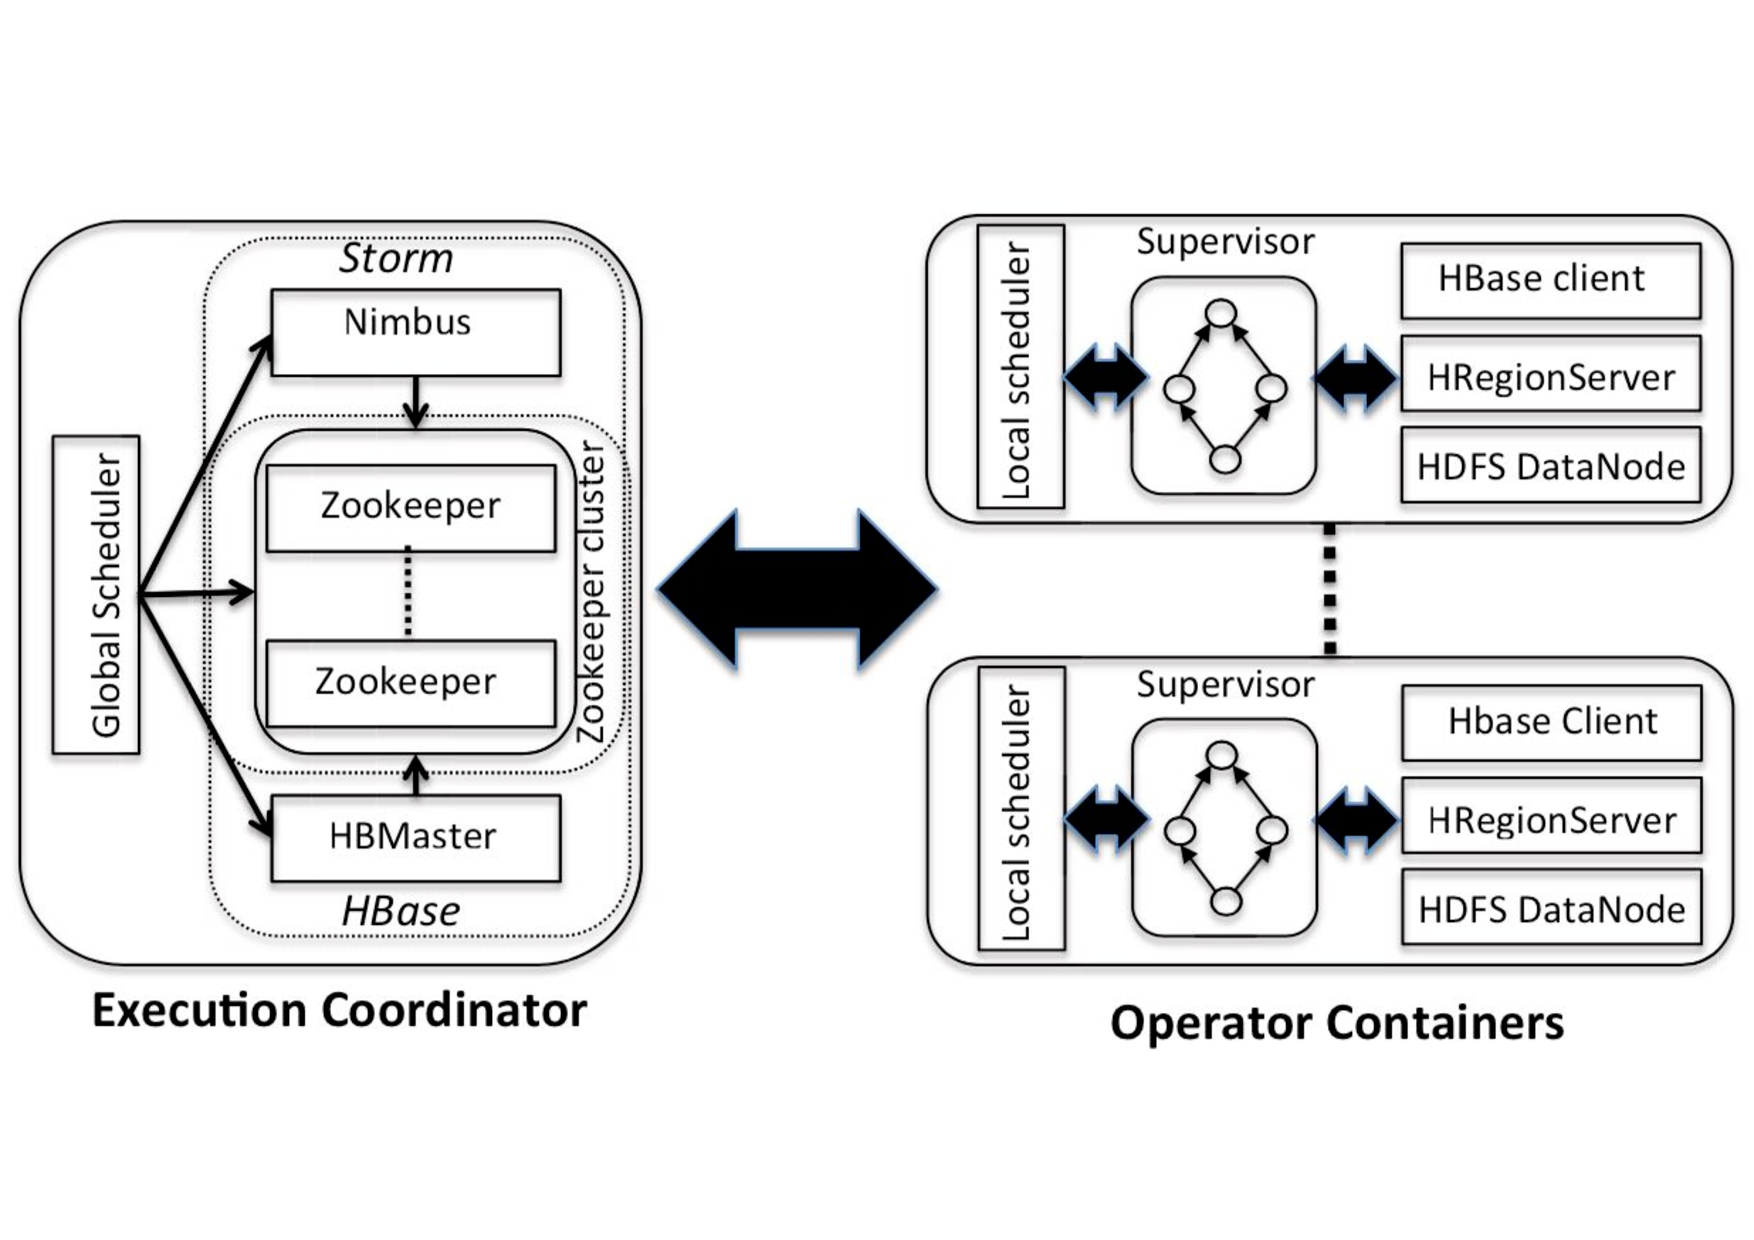
\includegraphics[width=0.85\textwidth]{img/cqels-cloud}
\caption{CQELS Cloud architecture (source~\cite{DBLP:conf/semweb/PhuocQVH13}).}
\label{fig:cqels-cloud}
\end{center}
\end{figure}

Figure~\ref{fig:cqels-cloud} depicts the general architecture of the system. CQELS Cloud implements the elastic execution model and the parallel algorithms exploiting ZooKeeper~\cite{DBLP:conf/usenix/HuntKJR10}, Storm\footnote{\url{http://storm-project.net/}} and HBase\footnote{\url{http://hbase.apache.org/}}. 

\paragraph{Strider}
Strider \cite{DBLP:conf/semweb/RenC17} is a distributed and adaptive RDF Stream Processing engine that optimizes logical query plan according to the data stream evolution developed to guarantee scalability, availability, fault-tolerance, high throughput and acceptable latency. 

Strider relies on well known distributed technology and is composed by two main components: (i) the data flow management and (ii) the Computing core. 
The former is based on Apache Kafka, it categorizes the input RDF streams into different message topics which represent the different family of RDF events.
The latter is based on the Spark Streaming framework, it creates a pipeline to perform parallel processing on the messages emitted by Kafka.

Strider proposes static and adaptive optimization components based, respectively, on heuristic rules and (stream-based) statistics and two strategies for the Adaptive Query Processing (AQP): backward (B-AQP) and forward (F-AQP) that mainly differ on the query plan computation time (i.e. at the previous or current window).

\section{RSP Middleware}\label{sec:rsp-mid}
RSP Middlewares ease the task of deploying the RSP Engine in real-world applications by offering extensible means for collecting data in real-time, for publishing, accessing and querying collected information as Linked Data, and for visualizing query results. 

In the next sections we present two different implementations of an RSP Middleware (the Streaming Linked Data (SLD) framework~\cite{DBLP:conf/semweb/BalduiniVDTPC13} and the Linked Stream Middleware~\cite{DBLP:journals/ws/PhuocNPH12}). They approach the problem in different ways. 
The SLD framework adopts a data driven in-memory approach for the processing of RDF streams with limited support for static information, the Linked Stream Middleware is a cloud-based infrastructure to integrate time-dependent data with other Linked Data sources. 

\subsection{Streaming Linked Data (SLD)} \label{sec:sld}
The Streaming Linked Data (SLD) framework is a general-purpose, pluggable system that supports the development of applications that continuously analyse RDF streams.
SLD is designed to address five different requirements:

\begin{itemize}
\item[\textbf{(R1)}] \emph{every input is an RDF data stream}. The system must indifferently ingest data with different velocities from any sources. All the incoming information is modeled as an RDF data stream. 
\item[\textbf{(R2)}] \emph{Continuous Ingestion}. The continuous nature of data streams requires a continuously capture phase. The data, once arrived, is marked with an increasing timestamp. The system could handle data arriving with its own time mark.
\item[\textbf{(R3)}] \emph{publish/subscribe}. SLD enable a publish/subscribe logic for its components. A senders, the \textsf{publishers}, publish timestamped RDF triples into RDF streams,  and receivers, the \textsf{subscribers}, listen to one or more RDF streams, and only receive timestamped RDF triples that are of their interest. Publisher and subscribers do not have to know each other.
\item[\textbf{(R4)}] \emph{reliable message-passing}. SLD implements a logically reliable message-passing system that guarantees timestamped RDF triples to be delivered in order.
\item[\textbf{(R5)}] \emph{minimizes latency by using main memory}. SLD minimizes latency by using main memory and avoiding disk I/O bottlenecks.
\end{itemize}

\begin{figure}[h]
\begin{center}
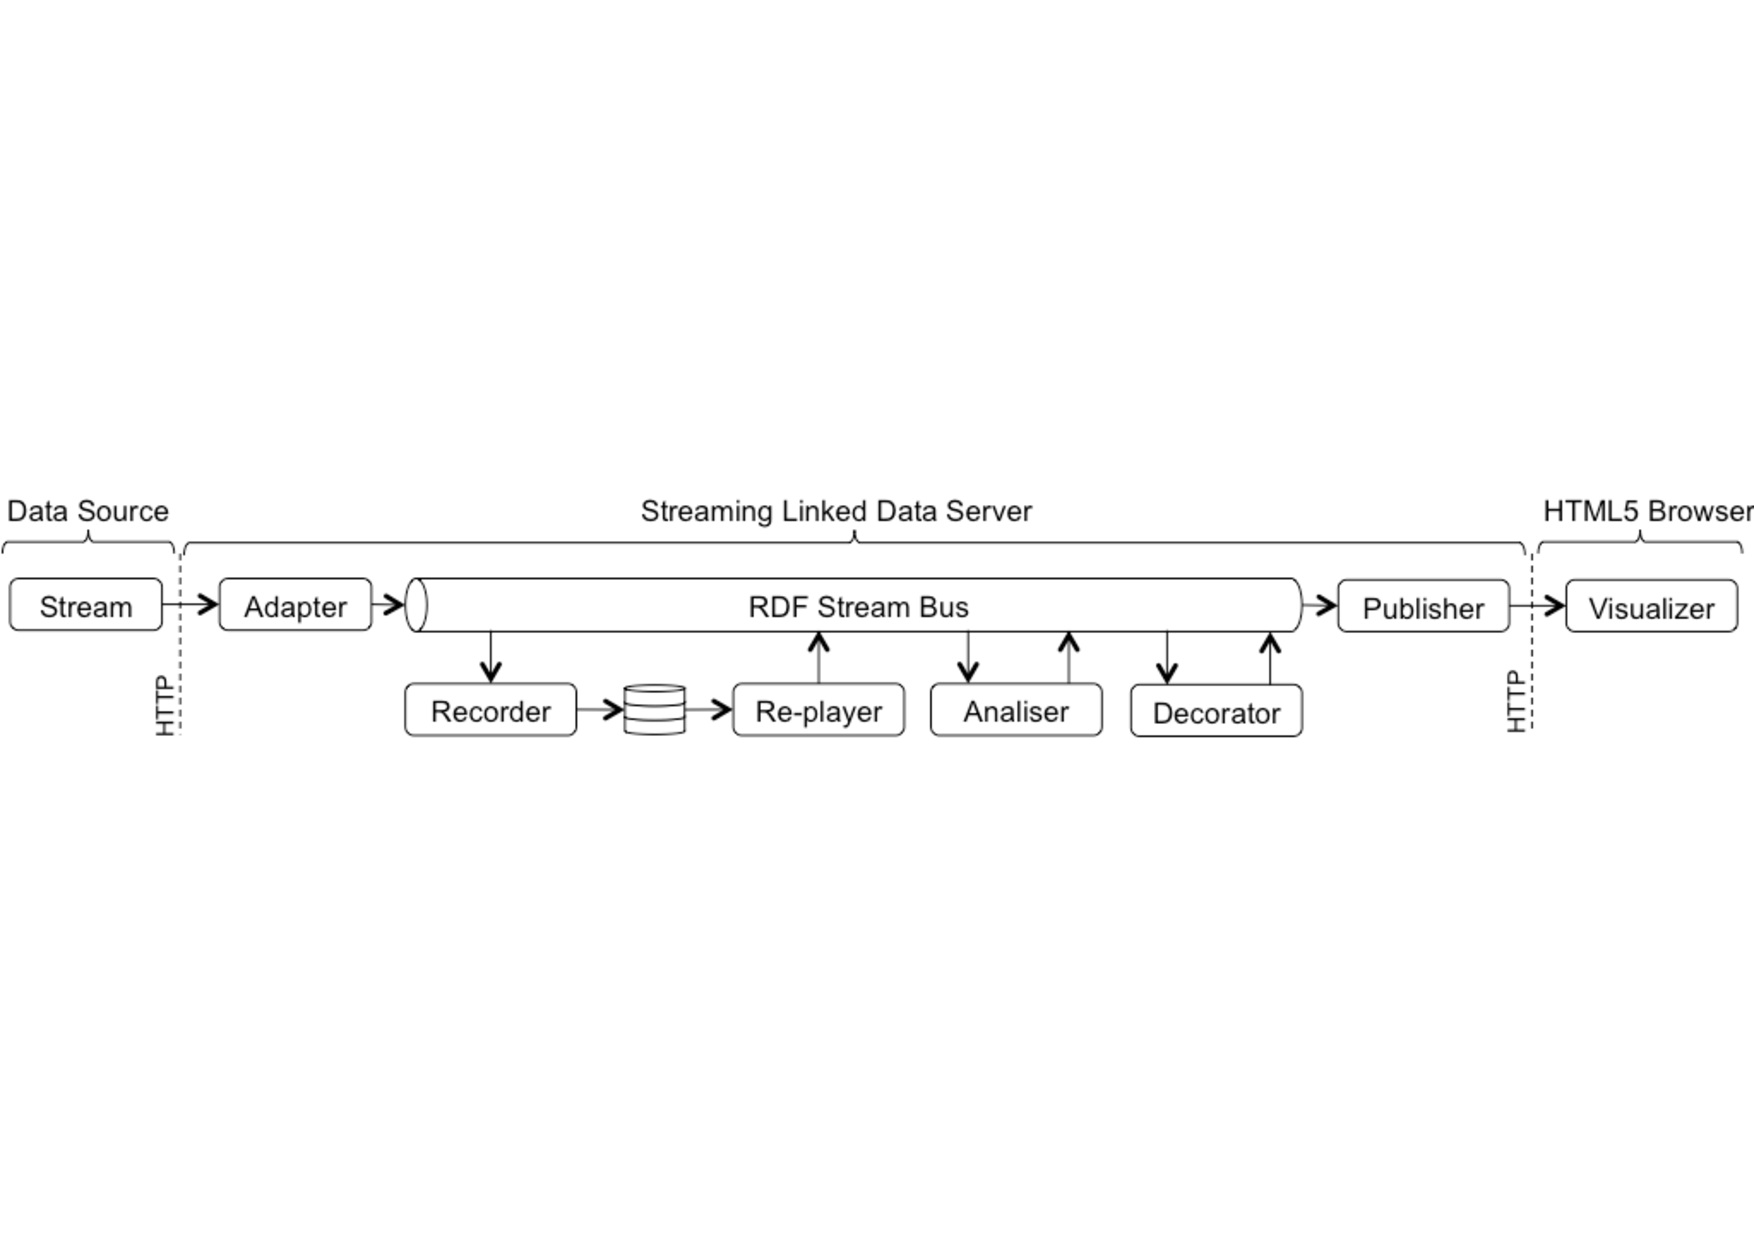
\includegraphics[width=1\textwidth]{img/SLD-arch}
\caption{The architecture of the Streaming Linked Data framework.}
\label{fig:sld-arch}
\end{center}
\end{figure}

Figure \ref{fig:sld-arch} illustrates the architecture of the SLD framework.  The leftmost column logically contains the \emph{streaming data sources}, the central one the SLD server, and the rightmost one the visual widgets to be embedded in a dashboard. 

The \emph{streaming data sources} are assumed to be distributed across the Web and accessible via HTTP.

The core of the framework is \emph{SLD Server}. It includes  components for accessing data stream sources, internally streaming data, registering and replaying portion of data streams,  decorating and analysing time-boxed portion of the stream, and publishing the results. 

The \textsf{adapters} allow to access data stream resources, possibly delegating filtering operations to the data source, and to translate data items in the stream into set of timestamped RDF triples. SLD framework includes adapters for different social networks (e.g., Twitter, Instagram, foursquare) and for several sensor networks. For instance, the Twitter adapter allows to push to Twitter either geo-spatial filters, which ask Twitter to stream to SLD only tweets posted from given locations, or keyword-based filters, which ask Twitter to stream to SLD only tweets containing one or more of such key-words. Each tweet is internally represented using the extension of SIOC ontology presented in \cite{DBLP:journals/ws/BalduiniCDVHLKT12}. 

The \textsf{publishers} make available on the Web the content of chosen RDF stream following the Linked Data principles \cite{DBLP:journals/ijswis/BizerHB09} in the Streaming Linked Data format proposed in \cite{DBLP:conf/www/BarbieriV10}. The format is based on two types of named RDF graphs: instantaneous Graphs (iGraphs), which contain a set triples having the same timestamp, and stream graphs (sGraphs), which contains triples that point to one or more timestamped iGraphs. The number of iGraphs pointed by an sGraph and their time interval of validity can be configured when instantiating the publisher.

The \textsf{recorders} are special types of publishers that allow for persistently storing a part of an RDF stream. As format, we used an extension of the Streaming Linked Data format based on iGraphs and recording graphs (rGraphs). The latter are similar to sGraphs, but they include pointers to all the iGraph recorded and such pointers do not have a time interval of validity. The \textsf{re-players} can inject in an RDF stream what recorded in an rGraph.

The \textsf{analysers} continuously observe the timestamped triples that flow in one or more RDF stream, perform analyses on them and generate a continuous stream of answers. SLD framework includes a built-in engine that executes C-SPARQL queries, but any of the aforementioned continuous extensions of SPARQL (see Section~\ref{sec:vel-var-solutions}) can be plugged in SLD server and used for the analysis. 

The \textsf{decorators} are special types of analysers that look for a pattern of triples in a RDF stream. When the pattern matches, the decorators run a computation of the matching and add new triples to the stream.

SLD represents the first attempts to create a streaming computational model with the definition of generic principles related to the RDF stream processing world. SLD inspires the generic streaming computational model presented in the Chapter~\ref{ch:computational}.

\subsection{Linked Stream Middleware}
Le-Phuoc et al.~\cite{DBLP:journals/ws/PhuocNPH12} proposes Linked Stream Middleware (LSM), a platform to create a bridge between data streams and Semantic Web.
LSM offers: (i) a wide range of extendable wrappers to access streaming sources and transform the raw data into Linked Stream Data~\cite{DBLP:conf/semweb/SequedaC09}, (ii) components for annotating and visualizing data through a Web interface and live querying functionalities over unified Linked Stream Data and data coming from the Linked Open Data cloud exploiting a standard SPARQL query processor and CQELS.

\begin{figure}[h]
\begin{center}
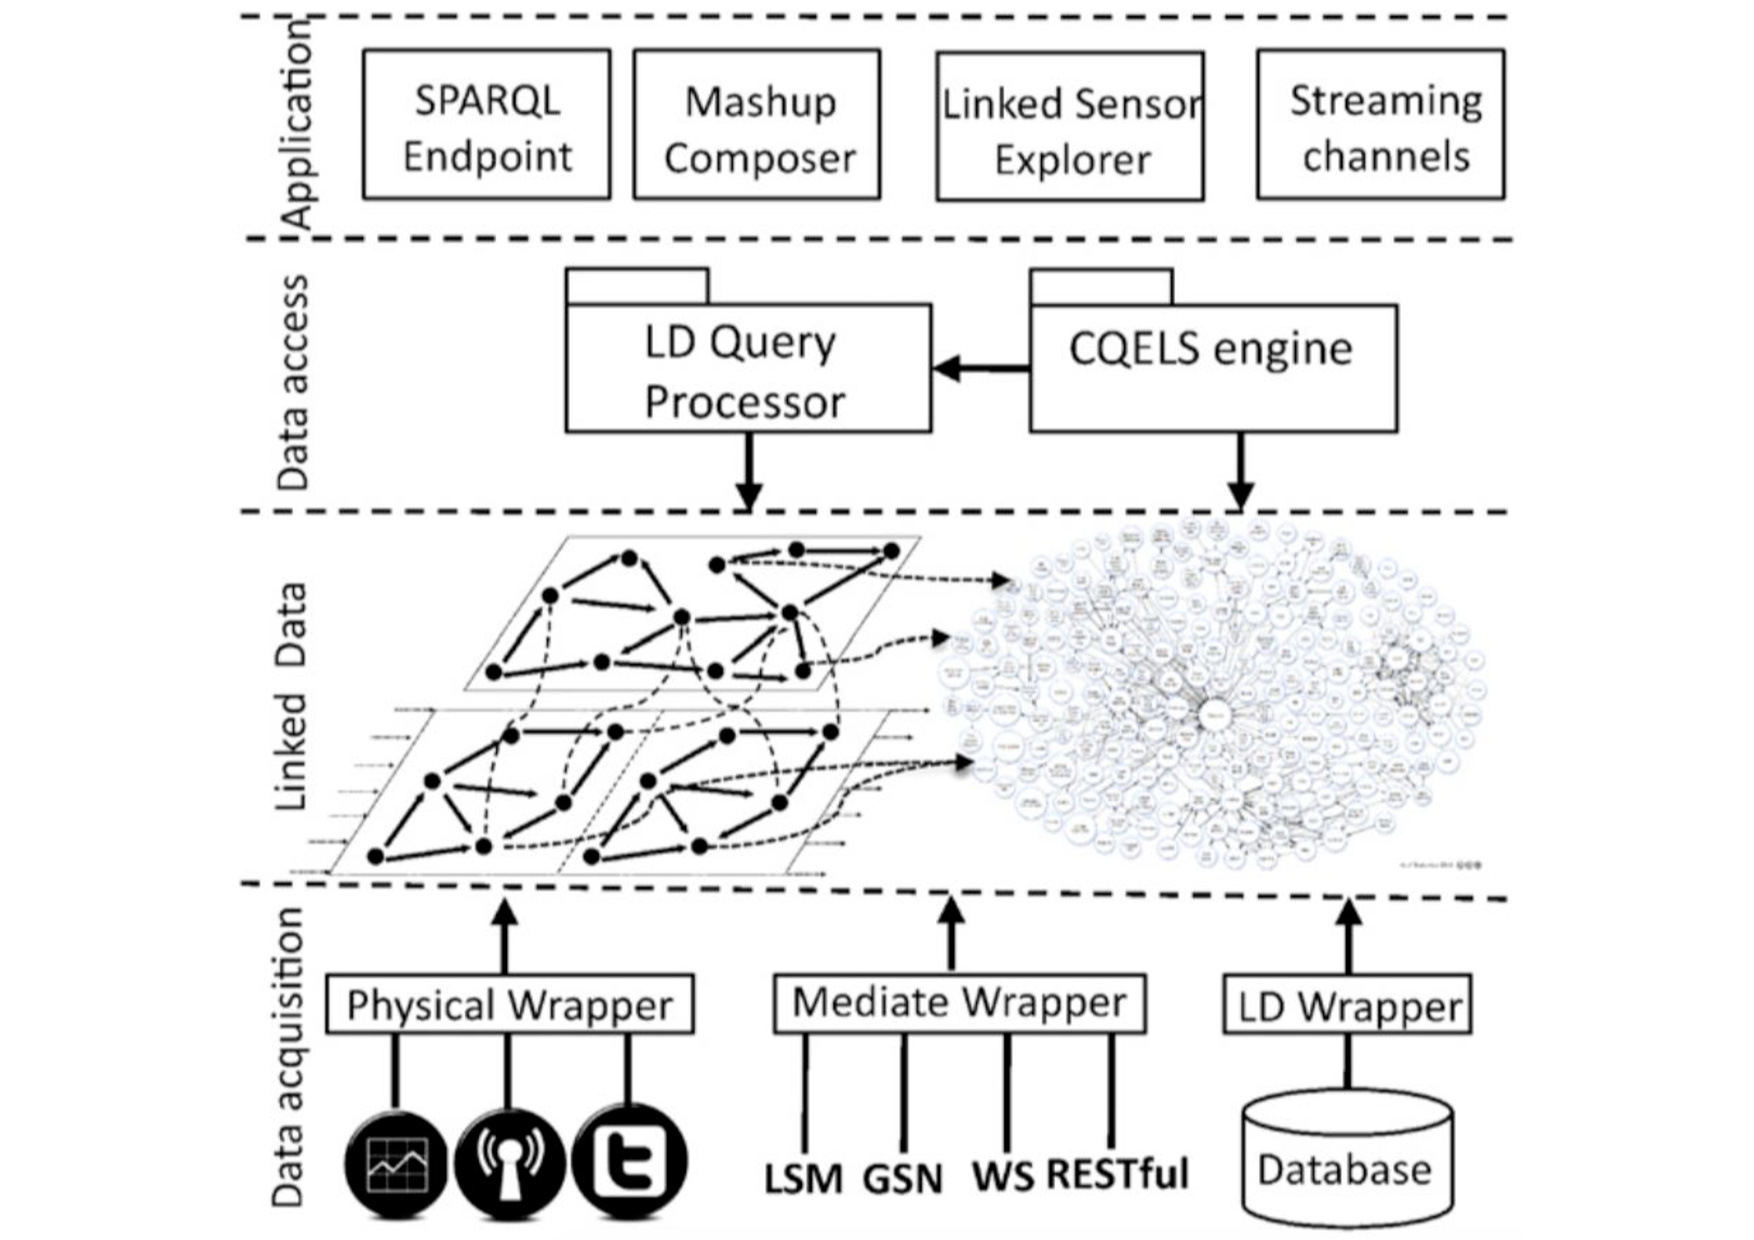
\includegraphics[width=0.7\textwidth]{img/lsm}
\caption{Linked Stream Middleware architecture (source~\cite{DBLP:journals/ws/PhuocNPH12})}
\label{fig:lsm-arch}
\end{center}
\end{figure}

The LSM architecture is layered to increase scalability and flexibility, Figure~\ref{fig:lsm-arch} presents an overview of LSM middleware.

The \textit{Data Acquisition layer} is in charge of collecting data from streaming data sources via a wide range of wrappers. The different characteristics of the proposed wrappers allows the system to cover a broad range of input format. The output of the wrappers conforms to format described in the Data Access Layer. The system allows users to develop their own wrapper in order to guarantee the flexibility of the entire system.
The \textit{Linked Data layer},  following the Linked Data publishing principles presented in~\cite{DBLP:series/synthesis/2011Heath},  adds a global identifier to the data to ensure the data composability and exploits an ontology to represent data in a triple-based format. In particular LSM use the Semantic Sensor Network (SSN) Ontology\footnote{\url{http://purl.oclc.org/NET/ssnx/ssn}}.
The \textit{Data Access layer} enable declarative query answering on top of the Linked Data layer  in a pull-based or push-based fashion. This layer enables the storage of stream data and metadata in a triple format to ease the access of historic data.
The \textit{Application layer} offers support for developing applications to exploit query processing capabilities of the Data Access layer. The layer offers a SPARQL Endpoint, a Linked Sensor Explorer, a Mashup Composer and Notifications/Stream channels and enables query operation on historical sensor data. Continuous queries can be registered into the system to populate user-defined output streams.

\section{Benchmarking}\label{sec:benchmarking}
In this section, we propose an overview the benchmarking principles. In particular, Section~\ref{sec:dsb} introduces \textit{domain-specific} benchmarks. Section~\ref{sec:vel-bench}, then, concentrates on the benchmarking of velocity oriented systems, i.e., systems created to deal with continuously flowing data (e.g., RSP). Finally, Section~\ref{sec:bench-cost} casts some light on the innovative concept of Configuration that Outperforms a Single Thread (COST), showing that a distributed solution, to be effective, must outperform a single-threaded one.


\subsection{Domain-Specific Benchmarks}\label{sec:dsb}
Nowadays, the variety of application of computer systems are growing faster than ever.
A single metric cannot measure and evaluate the performance of a computer system in all applications and domains.
A computer system is generally designed to face few problem domains and the performance in performing other tasks can be very poor.
Jim Gray~\cite{gray1992benchmark} proposes the \textit{domain-specific} benchmarks concept as a response to the heterogeneity of computer system use. 

A benchmark, built according to this concept, specifies a synthetic workload shaped to evaluate a system while it performs a typical application for which it was designed.
A \textit{domain-specific} benchmarks must follow four criteria. It must be: 
\begin{itemize}
\item \textit{Relevant}: given the problem domain, the benchmark must measure the peak performance and price/performance of the system during a typical domain-specific operation.
\item \textit{Portable}: the benchmark should be easy to be implemented on different systems and architectures.
\item \textit{Scalable}: the benchmark should apply to small and large computer systems, it should be also possible to test system on parallel architecture. 
\item \textit{Simple}: to ensure the credibility of the system, it must be understandable.
\end{itemize}

As stated in the principles, Gray \cite{gray1992benchmark} highlights the importance of price/performance metrics for system benchmarking.
The next sections will highlight the existing works on benchmarking streaming systems and the cost-aware approach.

\subsection{Benchmarking Velocity Oriented Systems}\label{sec:vel-bench}
The most relevant benchmark effort related to data stream management systems is the Linear Road benchmark~\cite{arasu2004linear}. In this work the authors present a benchmark specification for data management system with continuous querying capabilities. The benchmark is based on a traffic simulation use case. The system under test must answers queries from the vehicles on the road network in simulated real-time. The specification includes I/O, queries, expected results and relevant metrics for the system under test.

In many contexts, performance is very relevant. One of the first benchmarks for distributed streaming data processing is the Yahoo Streaming Benchmark~\cite{chintapalli2016benchmarking}.
This benchmark is based on a realistic use case. Also, a complete pipeline is implemented, from data ingestion to results. 
It is focused on performance metrics, namely latency and throughput, and it does not consider cost in its comparison. The benchmark code is available online under the Apache 2.0 license\footnote{https://github.com/yahoo/streaming-benchmarks}.

A more recent work on comparing popular distributed processing engines can be found in~\cite{karimov2018benchmarking}. This work presents a performance comparison for Apache Storm \cite{toshniwal2014storm}, Apache Flink \cite{carbone2015apache} and Apache Spark~\cite{zaharia2016apache}. The comparison is based on realistic industrial use cases, and it focuses on throughput and latency.

The correctness theme pushed the discussion on what is really important in a dsb for Stream Reasoning~\cite{DBLP:conf/esws/ScharrenbachUMVB13}.
Dell'Aglio et al.~\cite{DBLP:conf/semweb/DellAglioCBCV13} propose a formal characterization of the operational semantics of different RSP (i.e. C-SPARQL Engine, CQELS, SPARQL\textsubscript{stream} and EP-SPARQL) exploiting CQL and SECRET. This formalization allows to determine a concept of correctness in RSP domain and to develop CSRBench~\cite{DBLP:conf/semweb/DellAglioCBCV13} an extension of SRBench~\cite{DBLP:conf/semweb/ZhangDCC12} to address query result correctness verification using an automatic method.
Along the same line, Ali et al.~\cite{DBLP:conf/semweb/AliGM15} and Kolchin et al.~\cite{DBLP:conf/icwe/KolchinWKT16} propose workloads and software environments to run experiments and perform measurement of quality criteria.
A recent work of Tommasini et al.~\cite{DBLP:conf/esws/TommasiniVBD16} proposes an open-source test-stand to ensure the reproducibility of experiments.

The performance metrics plays a key role in the evaluation (see Section~\ref{sec:comp-mod-eval-performace}) of the implementations of our streaming Computational Model presented in Chapter~\ref{ch:computational}

\subsection{Cost-Aware approach}\label{sec:bench-cost}
Recently, in the Distributed System community, the concept of Configuration that Outperforms a Single Thread, namely COST, is gaining importance. 
McSherry et al.~\cite{mcsherry2015scalability} introduce the COST metric and demonstrate that a single-threaded implementation of popular graph algorithms outperforms all distributed graph processing engines by orders of magnitude, at a fraction of the cost. Similarly, Boden et al. \cite{bodendistributed} compare single-threaded implementations of common machine learning algorithms with their distributed counterparts. Those are implemented using the most popular distributed machine learning libraries.

The concept of COST plays a crucial role in the evaluation (see Chapter~\ref{sec:comp-mod-eval-cost}) of the different implementations of the Computational Model proposed in Chapter~\ref{ch:computational}




